\documentclass[twoside]{book}

% Packages required by doxygen
\usepackage{fixltx2e}
\usepackage{calc}
\usepackage{doxygen}
\usepackage[export]{adjustbox} % also loads graphicx
\usepackage{graphicx}
\usepackage[utf8]{inputenc}
\usepackage{makeidx}
\usepackage{multicol}
\usepackage{multirow}
\PassOptionsToPackage{warn}{textcomp}
\usepackage{textcomp}
\usepackage[nointegrals]{wasysym}
\usepackage[table]{xcolor}

% Font selection
\usepackage[T1]{fontenc}
\usepackage[scaled=.90]{helvet}
\usepackage{courier}
\usepackage{amssymb}
\usepackage{sectsty}
\renewcommand{\familydefault}{\sfdefault}
\allsectionsfont{%
  \fontseries{bc}\selectfont%
  \color{darkgray}%
}
\renewcommand{\DoxyLabelFont}{%
  \fontseries{bc}\selectfont%
  \color{darkgray}%
}
\newcommand{\+}{\discretionary{\mbox{\scriptsize$\hookleftarrow$}}{}{}}

% Page & text layout
\usepackage{geometry}
\geometry{%
  a4paper,%
  top=2.5cm,%
  bottom=2.5cm,%
  left=2.5cm,%
  right=2.5cm%
}
\tolerance=750
\hfuzz=15pt
\hbadness=750
\setlength{\emergencystretch}{15pt}
\setlength{\parindent}{0cm}
\setlength{\parskip}{3ex plus 2ex minus 2ex}
\makeatletter
\renewcommand{\paragraph}{%
  \@startsection{paragraph}{4}{0ex}{-1.0ex}{1.0ex}{%
    \normalfont\normalsize\bfseries\SS@parafont%
  }%
}
\renewcommand{\subparagraph}{%
  \@startsection{subparagraph}{5}{0ex}{-1.0ex}{1.0ex}{%
    \normalfont\normalsize\bfseries\SS@subparafont%
  }%
}
\makeatother

% Headers & footers
\usepackage{fancyhdr}
\pagestyle{fancyplain}
\fancyhead[LE]{\fancyplain{}{\bfseries\thepage}}
\fancyhead[CE]{\fancyplain{}{}}
\fancyhead[RE]{\fancyplain{}{\bfseries\leftmark}}
\fancyhead[LO]{\fancyplain{}{\bfseries\rightmark}}
\fancyhead[CO]{\fancyplain{}{}}
\fancyhead[RO]{\fancyplain{}{\bfseries\thepage}}
\fancyfoot[LE]{\fancyplain{}{}}
\fancyfoot[CE]{\fancyplain{}{}}
\fancyfoot[RE]{\fancyplain{}{\bfseries\scriptsize Generated by Doxygen }}
\fancyfoot[LO]{\fancyplain{}{\bfseries\scriptsize Generated by Doxygen }}
\fancyfoot[CO]{\fancyplain{}{}}
\fancyfoot[RO]{\fancyplain{}{}}
\renewcommand{\footrulewidth}{0.4pt}
\renewcommand{\chaptermark}[1]{%
  \markboth{#1}{}%
}
\renewcommand{\sectionmark}[1]{%
  \markright{\thesection\ #1}%
}

% Indices & bibliography
\usepackage{natbib}
\usepackage[titles]{tocloft}
\setcounter{tocdepth}{3}
\setcounter{secnumdepth}{5}
\makeindex

% Hyperlinks (required, but should be loaded last)
\usepackage{ifpdf}
\ifpdf
  \usepackage[pdftex,pagebackref=true]{hyperref}
\else
  \usepackage[ps2pdf,pagebackref=true]{hyperref}
\fi
\hypersetup{%
  colorlinks=true,%
  linkcolor=blue,%
  citecolor=blue,%
  unicode%
}

% Custom commands
\newcommand{\clearemptydoublepage}{%
  \newpage{\pagestyle{empty}\cleardoublepage}%
}

\usepackage{caption}
\captionsetup{labelsep=space,justification=centering,font={bf},singlelinecheck=off,skip=4pt,position=top}

%===== C O N T E N T S =====

\begin{document}

% Titlepage & ToC
\hypersetup{pageanchor=false,
             bookmarksnumbered=true,
             pdfencoding=unicode
            }
\pagenumbering{alph}
\begin{titlepage}
\vspace*{7cm}
\begin{center}%
{\Large My Project }\\
\vspace*{1cm}
{\large Generated by Doxygen 1.8.14}\\
\end{center}
\end{titlepage}
\clearemptydoublepage
\pagenumbering{roman}
\tableofcontents
\clearemptydoublepage
\pagenumbering{arabic}
\hypersetup{pageanchor=true}

%--- Begin generated contents ---
\chapter{Namespace Index}
\section{Namespace List}
Here is a list of all namespaces with brief descriptions\+:\begin{DoxyCompactList}
\item\contentsline{section}{\mbox{\hyperlink{namespace_configuracion}{Configuracion}} }{\pageref{namespace_configuracion}}{}
\item\contentsline{section}{\mbox{\hyperlink{namespace_control}{Control}} }{\pageref{namespace_control}}{}
\item\contentsline{section}{\mbox{\hyperlink{namespace_dao_b_d_paciente}{Dao\+B\+D\+Paciente}} }{\pageref{namespace_dao_b_d_paciente}}{}
\item\contentsline{section}{\mbox{\hyperlink{namespace_dao_b_d_usuario}{Dao\+B\+D\+Usuario}} }{\pageref{namespace_dao_b_d_usuario}}{}
\item\contentsline{section}{\mbox{\hyperlink{namespace_dao_d_b_muestra}{Dao\+D\+B\+Muestra}} }{\pageref{namespace_dao_d_b_muestra}}{}
\item\contentsline{section}{\mbox{\hyperlink{namespace_d_t_o_paciente}{D\+T\+O\+Paciente}} }{\pageref{namespace_d_t_o_paciente}}{}
\item\contentsline{section}{\mbox{\hyperlink{namespace_facade}{Facade}} }{\pageref{namespace_facade}}{}
\item\contentsline{section}{\mbox{\hyperlink{namespace_facade_administrador}{Facade\+Administrador}} }{\pageref{namespace_facade_administrador}}{}
\item\contentsline{section}{\mbox{\hyperlink{namespace_facede_medico}{Facede\+Medico}} }{\pageref{namespace_facede_medico}}{}
\item\contentsline{section}{\mbox{\hyperlink{namespace_gestor_muestra}{Gestor\+Muestra}} }{\pageref{namespace_gestor_muestra}}{}
\item\contentsline{section}{\mbox{\hyperlink{namespace_gestor_paciente}{Gestor\+Paciente}} }{\pageref{namespace_gestor_paciente}}{}
\item\contentsline{section}{\mbox{\hyperlink{namespace_imagen}{Imagen}} }{\pageref{namespace_imagen}}{}
\item\contentsline{section}{\mbox{\hyperlink{namespace_m_a_e}{M\+AE}} }{\pageref{namespace_m_a_e}}{}
\item\contentsline{section}{\mbox{\hyperlink{namespace_m_s_e}{M\+SE}} }{\pageref{namespace_m_s_e}}{}
\item\contentsline{section}{\mbox{\hyperlink{namespace_muestra}{Muestra}} }{\pageref{namespace_muestra}}{}
\item\contentsline{section}{\mbox{\hyperlink{namespace_paciente}{Paciente}} }{\pageref{namespace_paciente}}{}
\item\contentsline{section}{\mbox{\hyperlink{namespace_prueba}{Prueba}} }{\pageref{namespace_prueba}}{}
\item\contentsline{section}{\mbox{\hyperlink{namespace_r_e_d}{R\+ED}} }{\pageref{namespace_r_e_d}}{}
\item\contentsline{section}{\mbox{\hyperlink{namespace_u_i_usuario}{U\+I\+Usuario}} }{\pageref{namespace_u_i_usuario}}{}
\end{DoxyCompactList}

\chapter{Hierarchical Index}
\section{Class Hierarchy}
This inheritance list is sorted roughly, but not completely, alphabetically\+:\begin{DoxyCompactList}
\item \contentsline{section}{Configuracion.\+Configuracion}{\pageref{class_configuracion_1_1_configuracion}}{}
\item \contentsline{section}{Control.\+Control}{\pageref{class_control_1_1_control}}{}
\item \contentsline{section}{Facade.\+Facade}{\pageref{class_facade_1_1_facade}}{}
\begin{DoxyCompactList}
\item \contentsline{section}{Facade\+Administrador.\+Facade\+Administrador}{\pageref{class_facade_administrador_1_1_facade_administrador}}{}
\item \contentsline{section}{Facede\+Medico.\+Facade\+Medico}{\pageref{class_facede_medico_1_1_facade_medico}}{}
\end{DoxyCompactList}
\item \contentsline{section}{U\+I\+Usuario.\+U\+I\+Usuario}{\pageref{class_u_i_usuario_1_1_u_i_usuario}}{}
\end{DoxyCompactList}

\chapter{Class Index}
\section{Class List}
Here are the classes, structs, unions and interfaces with brief descriptions\+:\begin{DoxyCompactList}
\item\contentsline{section}{\mbox{\hyperlink{class_configuracion_1_1_configuracion}{Configuracion.\+Configuracion}} }{\pageref{class_configuracion_1_1_configuracion}}{}
\item\contentsline{section}{\mbox{\hyperlink{class_control_1_1_control}{Control.\+Control}} \\*Documentation for a class }{\pageref{class_control_1_1_control}}{}
\item\contentsline{section}{\mbox{\hyperlink{class_dao_b_d_paciente_1_1_dao_b_d_paciente}{Dao\+B\+D\+Paciente.\+Dao\+B\+D\+Paciente}} \\*Documentation for a class }{\pageref{class_dao_b_d_paciente_1_1_dao_b_d_paciente}}{}
\item\contentsline{section}{\mbox{\hyperlink{class_dao_b_d_usuario_1_1_dao_b_d_usuario}{Dao\+B\+D\+Usuario.\+Dao\+B\+D\+Usuario}} \\*Documentation for a class }{\pageref{class_dao_b_d_usuario_1_1_dao_b_d_usuario}}{}
\item\contentsline{section}{\mbox{\hyperlink{class_dao_d_b_muestra_1_1_dao_d_b_muestra}{Dao\+D\+B\+Muestra.\+Dao\+D\+B\+Muestra}} \\*Documentation for a class }{\pageref{class_dao_d_b_muestra_1_1_dao_d_b_muestra}}{}
\item\contentsline{section}{\mbox{\hyperlink{class_d_t_o_paciente_1_1_d_t_o_paciente}{D\+T\+O\+Paciente.\+D\+T\+O\+Paciente}} \\*Documentation for a class }{\pageref{class_d_t_o_paciente_1_1_d_t_o_paciente}}{}
\item\contentsline{section}{\mbox{\hyperlink{class_facade_1_1_facade}{Facade.\+Facade}} \\*Documentation for a class }{\pageref{class_facade_1_1_facade}}{}
\item\contentsline{section}{\mbox{\hyperlink{class_facade_administrador_1_1_facade_administrador}{Facade\+Administrador.\+Facade\+Administrador}} }{\pageref{class_facade_administrador_1_1_facade_administrador}}{}
\item\contentsline{section}{\mbox{\hyperlink{class_facede_medico_1_1_facade_medico}{Facede\+Medico.\+Facade\+Medico}} }{\pageref{class_facede_medico_1_1_facade_medico}}{}
\item\contentsline{section}{\mbox{\hyperlink{class_gestor_muestra_1_1_gestor_muestra}{Gestor\+Muestra.\+Gestor\+Muestra}} }{\pageref{class_gestor_muestra_1_1_gestor_muestra}}{}
\item\contentsline{section}{\mbox{\hyperlink{class_gestor_paciente_1_1_gestor_paciente}{Gestor\+Paciente.\+Gestor\+Paciente}} }{\pageref{class_gestor_paciente_1_1_gestor_paciente}}{}
\item\contentsline{section}{\mbox{\hyperlink{class_imagen_1_1_imagen}{Imagen.\+Imagen}} }{\pageref{class_imagen_1_1_imagen}}{}
\item\contentsline{section}{\mbox{\hyperlink{class_m_a_e_1_1_m_a_e}{M\+A\+E.\+M\+AE}} }{\pageref{class_m_a_e_1_1_m_a_e}}{}
\item\contentsline{section}{\mbox{\hyperlink{class_m_s_e_1_1_m_s_e}{M\+S\+E.\+M\+SE}} }{\pageref{class_m_s_e_1_1_m_s_e}}{}
\item\contentsline{section}{\mbox{\hyperlink{class_muestra_1_1_muestra}{Muestra.\+Muestra}} }{\pageref{class_muestra_1_1_muestra}}{}
\item\contentsline{section}{\mbox{\hyperlink{class_paciente_1_1_paciente}{Paciente.\+Paciente}} }{\pageref{class_paciente_1_1_paciente}}{}
\item\contentsline{section}{\mbox{\hyperlink{class_prueba_1_1_prueba}{Prueba.\+Prueba}} }{\pageref{class_prueba_1_1_prueba}}{}
\item\contentsline{section}{\mbox{\hyperlink{class_r_e_d_1_1_r_e_d}{R\+E\+D.\+R\+ED}} }{\pageref{class_r_e_d_1_1_r_e_d}}{}
\item\contentsline{section}{\mbox{\hyperlink{class_u_i_usuario_1_1_u_i_usuario}{U\+I\+Usuario.\+U\+I\+Usuario}} }{\pageref{class_u_i_usuario_1_1_u_i_usuario}}{}
\end{DoxyCompactList}

\chapter{File Index}
\section{File List}
Here is a list of all files with brief descriptions\+:\begin{DoxyCompactList}
\item\contentsline{section}{control/\mbox{\hyperlink{_configuracion_8py}{Configuracion.\+py}} }{\pageref{_configuracion_8py}}{}
\item\contentsline{section}{control/\mbox{\hyperlink{_control_8py}{Control.\+py}} }{\pageref{_control_8py}}{}
\item\contentsline{section}{control/\mbox{\hyperlink{_dao_b_d_paciente_8py}{Dao\+B\+D\+Paciente.\+py}} }{\pageref{_dao_b_d_paciente_8py}}{}
\item\contentsline{section}{control/\mbox{\hyperlink{_dao_b_d_usuario_8py}{Dao\+B\+D\+Usuario.\+py}} }{\pageref{_dao_b_d_usuario_8py}}{}
\item\contentsline{section}{control/\mbox{\hyperlink{_dao_d_b_muestra_8py}{Dao\+D\+B\+Muestra.\+py}} }{\pageref{_dao_d_b_muestra_8py}}{}
\item\contentsline{section}{control/\mbox{\hyperlink{_d_t_o_paciente_8py}{D\+T\+O\+Paciente.\+py}} }{\pageref{_d_t_o_paciente_8py}}{}
\item\contentsline{section}{control/\mbox{\hyperlink{_facade_8py}{Facade.\+py}} }{\pageref{_facade_8py}}{}
\item\contentsline{section}{control/\mbox{\hyperlink{_facade_administrador_8py}{Facade\+Administrador.\+py}} }{\pageref{_facade_administrador_8py}}{}
\item\contentsline{section}{control/\mbox{\hyperlink{_facede_medico_8py}{Facede\+Medico.\+py}} }{\pageref{_facede_medico_8py}}{}
\item\contentsline{section}{control/\mbox{\hyperlink{_gestor_muestra_8py}{Gestor\+Muestra.\+py}} }{\pageref{_gestor_muestra_8py}}{}
\item\contentsline{section}{control/\mbox{\hyperlink{_gestor_paciente_8py}{Gestor\+Paciente.\+py}} }{\pageref{_gestor_paciente_8py}}{}
\item\contentsline{section}{control/\mbox{\hyperlink{_u_i_usuario_8py}{U\+I\+Usuario.\+py}} }{\pageref{_u_i_usuario_8py}}{}
\item\contentsline{section}{modelo/\mbox{\hyperlink{_imagen_8py}{Imagen.\+py}} }{\pageref{_imagen_8py}}{}
\item\contentsline{section}{modelo/\mbox{\hyperlink{_m_a_e_8py}{M\+A\+E.\+py}} }{\pageref{_m_a_e_8py}}{}
\item\contentsline{section}{modelo/\mbox{\hyperlink{_m_s_e_8py}{M\+S\+E.\+py}} }{\pageref{_m_s_e_8py}}{}
\item\contentsline{section}{modelo/\mbox{\hyperlink{_muestra_8py}{Muestra.\+py}} }{\pageref{_muestra_8py}}{}
\item\contentsline{section}{modelo/\mbox{\hyperlink{_paciente_8py}{Paciente.\+py}} }{\pageref{_paciente_8py}}{}
\item\contentsline{section}{modelo/\mbox{\hyperlink{_prueba_8py}{Prueba.\+py}} }{\pageref{_prueba_8py}}{}
\item\contentsline{section}{modelo/\mbox{\hyperlink{_r_e_d_8py}{R\+E\+D.\+py}} }{\pageref{_r_e_d_8py}}{}
\end{DoxyCompactList}

\chapter{Namespace Documentation}
\hypertarget{namespace_configuracion}{}\section{Configuracion Namespace Reference}
\label{namespace_configuracion}\index{Configuracion@{Configuracion}}
\subsection*{Classes}
\begin{DoxyCompactItemize}
\item 
class \mbox{\hyperlink{class_configuracion_1_1_configuracion}{Configuracion}}
\end{DoxyCompactItemize}

\hypertarget{namespace_control}{}\section{Control Namespace Reference}
\label{namespace_control}\index{Control@{Control}}
\subsection*{Classes}
\begin{DoxyCompactItemize}
\item 
class \mbox{\hyperlink{class_control_1_1_control}{Control}}
\begin{DoxyCompactList}\small\item\em Documentation for a class. \end{DoxyCompactList}\end{DoxyCompactItemize}

\hypertarget{namespace_dao_b_d_paciente}{}\section{Dao\+B\+D\+Paciente Namespace Reference}
\label{namespace_dao_b_d_paciente}\index{Dao\+B\+D\+Paciente@{Dao\+B\+D\+Paciente}}

\hypertarget{namespace_dao_b_d_usuario}{}\section{Dao\+B\+D\+Usuario Namespace Reference}
\label{namespace_dao_b_d_usuario}\index{Dao\+B\+D\+Usuario@{Dao\+B\+D\+Usuario}}
\subsection*{Classes}
\begin{DoxyCompactItemize}
\item 
class \mbox{\hyperlink{class_dao_b_d_usuario_1_1_dao_b_d_usuario}{Dao\+B\+D\+Usuario}}
\begin{DoxyCompactList}\small\item\em Documentation for a class. \end{DoxyCompactList}\end{DoxyCompactItemize}

\hypertarget{namespace_dao_d_b_muestra}{}\section{Dao\+D\+B\+Muestra Namespace Reference}
\label{namespace_dao_d_b_muestra}\index{Dao\+D\+B\+Muestra@{Dao\+D\+B\+Muestra}}

\hypertarget{namespace_d_t_o_paciente}{}\section{D\+T\+O\+Paciente Namespace Reference}
\label{namespace_d_t_o_paciente}\index{D\+T\+O\+Paciente@{D\+T\+O\+Paciente}}
\subsection*{Classes}
\begin{DoxyCompactItemize}
\item 
class \mbox{\hyperlink{class_d_t_o_paciente_1_1_d_t_o_paciente}{D\+T\+O\+Paciente}}
\begin{DoxyCompactList}\small\item\em Documentation for a class. \end{DoxyCompactList}\end{DoxyCompactItemize}

\hypertarget{namespace_estimador}{}\section{Estimador Namespace Reference}
\label{namespace_estimador}\index{Estimador@{Estimador}}
\subsection*{Classes}
\begin{DoxyCompactItemize}
\item 
class \mbox{\hyperlink{class_estimador_1_1_estimador}{Estimador}}
\begin{DoxyCompactList}\small\item\em Documentation for a class. \end{DoxyCompactList}\end{DoxyCompactItemize}

\hypertarget{namespace_facade}{}\section{Facade Namespace Reference}
\label{namespace_facade}\index{Facade@{Facade}}
\subsection*{Classes}
\begin{DoxyCompactItemize}
\item 
class \mbox{\hyperlink{class_facade_1_1_facade}{Facade}}
\end{DoxyCompactItemize}

\hypertarget{namespace_facade_administrador}{}\section{Facade\+Administrador Namespace Reference}
\label{namespace_facade_administrador}\index{Facade\+Administrador@{Facade\+Administrador}}
\subsection*{Classes}
\begin{DoxyCompactItemize}
\item 
class \mbox{\hyperlink{class_facade_administrador_1_1_facade_administrador}{Facade\+Administrador}}
\begin{DoxyCompactList}\small\item\em Documentation for a class. \end{DoxyCompactList}\end{DoxyCompactItemize}

\hypertarget{namespace_facede_medico}{}\section{Facede\+Medico Namespace Reference}
\label{namespace_facede_medico}\index{Facede\+Medico@{Facede\+Medico}}
\subsection*{Classes}
\begin{DoxyCompactItemize}
\item 
class \mbox{\hyperlink{class_facede_medico_1_1_facade_medico}{Facade\+Medico}}
\end{DoxyCompactItemize}

\hypertarget{namespace_gestor_muestra}{}\section{Gestor\+Muestra Namespace Reference}
\label{namespace_gestor_muestra}\index{Gestor\+Muestra@{Gestor\+Muestra}}
\subsection*{Classes}
\begin{DoxyCompactItemize}
\item 
class \mbox{\hyperlink{class_gestor_muestra_1_1_gestor_muestra}{Gestor\+Muestra}}
\end{DoxyCompactItemize}

\hypertarget{namespace_gestor_paciente}{}\section{Gestor\+Paciente Namespace Reference}
\label{namespace_gestor_paciente}\index{Gestor\+Paciente@{Gestor\+Paciente}}
\subsection*{Classes}
\begin{DoxyCompactItemize}
\item 
class \mbox{\hyperlink{class_gestor_paciente_1_1_gestor_paciente}{Gestor\+Paciente}}
\end{DoxyCompactItemize}

\hypertarget{namespace_imagen}{}\section{Imagen Namespace Reference}
\label{namespace_imagen}\index{Imagen@{Imagen}}
\subsection*{Classes}
\begin{DoxyCompactItemize}
\item 
class \mbox{\hyperlink{class_imagen_1_1_imagen}{Imagen}}
\begin{DoxyCompactList}\small\item\em Documentation for a class. \end{DoxyCompactList}\end{DoxyCompactItemize}

\hypertarget{namespace_m_a_e}{}\section{M\+AE Namespace Reference}
\label{namespace_m_a_e}\index{M\+AE@{M\+AE}}

\hypertarget{namespacemodelo}{}\section{modelo Namespace Reference}
\label{namespacemodelo}\index{modelo@{modelo}}

\hypertarget{namespace_m_s_e}{}\section{M\+SE Namespace Reference}
\label{namespace_m_s_e}\index{M\+SE@{M\+SE}}
\subsection*{Classes}
\begin{DoxyCompactItemize}
\item 
class \mbox{\hyperlink{class_m_s_e_1_1_m_s_e}{M\+SE}}
\end{DoxyCompactItemize}

\hypertarget{namespace_muestra}{}\section{Muestra Namespace Reference}
\label{namespace_muestra}\index{Muestra@{Muestra}}
\subsection*{Classes}
\begin{DoxyCompactItemize}
\item 
class \mbox{\hyperlink{class_muestra_1_1_muestra}{Muestra}}
\end{DoxyCompactItemize}

\hypertarget{namespace_paciente}{}\section{Paciente Namespace Reference}
\label{namespace_paciente}\index{Paciente@{Paciente}}

\hypertarget{namespace_prueba}{}\section{Prueba Namespace Reference}
\label{namespace_prueba}\index{Prueba@{Prueba}}
\subsection*{Classes}
\begin{DoxyCompactItemize}
\item 
class \mbox{\hyperlink{class_prueba_1_1_prueba}{Prueba}}
\begin{DoxyCompactList}\small\item\em Documentation for a class. \end{DoxyCompactList}\end{DoxyCompactItemize}

\hypertarget{namespace_u_i_usuario}{}\section{U\+I\+Usuario Namespace Reference}
\label{namespace_u_i_usuario}\index{U\+I\+Usuario@{U\+I\+Usuario}}
\subsection*{Classes}
\begin{DoxyCompactItemize}
\item 
class \mbox{\hyperlink{class_u_i_usuario_1_1_u_i_usuario}{U\+I\+Usuario}}
\begin{DoxyCompactList}\small\item\em Documentation for a class. \end{DoxyCompactList}\end{DoxyCompactItemize}

\chapter{Class Documentation}
\hypertarget{class_configuracion_1_1_configuracion}{}\section{Configuracion.\+Configuracion Class Reference}
\label{class_configuracion_1_1_configuracion}\index{Configuracion.\+Configuracion@{Configuracion.\+Configuracion}}
\subsection*{Static Public Attributes}
\begin{DoxyCompactItemize}
\item 
\mbox{\hyperlink{class_configuracion_1_1_configuracion_a8aed3273377e5707e9a22f395d5562e9}{D\+I\+R\+E\+C\+C\+I\+ON}} = os.\+path.\+split(os.\+path.\+abspath(\+\_\+\+\_\+file\+\_\+\+\_\+))\mbox{[}0\mbox{]}
\end{DoxyCompactItemize}


\subsection{Member Data Documentation}
\mbox{\Hypertarget{class_configuracion_1_1_configuracion_a8aed3273377e5707e9a22f395d5562e9}\label{class_configuracion_1_1_configuracion_a8aed3273377e5707e9a22f395d5562e9}} 
\index{Configuracion\+::\+Configuracion@{Configuracion\+::\+Configuracion}!D\+I\+R\+E\+C\+C\+I\+ON@{D\+I\+R\+E\+C\+C\+I\+ON}}
\index{D\+I\+R\+E\+C\+C\+I\+ON@{D\+I\+R\+E\+C\+C\+I\+ON}!Configuracion\+::\+Configuracion@{Configuracion\+::\+Configuracion}}
\subsubsection{\texorpdfstring{D\+I\+R\+E\+C\+C\+I\+ON}{DIRECCION}}
{\footnotesize\ttfamily Configuracion.\+Configuracion.\+D\+I\+R\+E\+C\+C\+I\+ON = os.\+path.\+split(os.\+path.\+abspath(\+\_\+\+\_\+file\+\_\+\+\_\+))\mbox{[}0\mbox{]}\hspace{0.3cm}{\ttfamily [static]}}



The documentation for this class was generated from the following file\+:\begin{DoxyCompactItemize}
\item 
C\+:/\+Users/olman/\+Documents/\+Git\+Hub/\+A\+S\+C-\/\+Proyecto-\/\+I\+S-\/2018/website/main/back\+\_\+end/control/\mbox{\hyperlink{_configuracion_8py}{Configuracion.\+py}}\end{DoxyCompactItemize}

\hypertarget{class_control_1_1_control}{}\section{Control.\+Control Class Reference}
\label{class_control_1_1_control}\index{Control.\+Control@{Control.\+Control}}


Documentation for a class.  


\subsection*{Public Member Functions}
\begin{DoxyCompactItemize}
\item 
def \mbox{\hyperlink{class_control_1_1_control_acbf9737a141c25fda2909c24f68cb75e}{\+\_\+\+\_\+init\+\_\+\+\_\+}} (self)
\item 
def \mbox{\hyperlink{class_control_1_1_control_aae955f5fe750e5f2d2764ff3893b75f5}{cargar\+\_\+imagen}} (self, nombre)
\begin{DoxyCompactList}\small\item\em Documentation Cargar imagen. \end{DoxyCompactList}\item 
def \mbox{\hyperlink{class_control_1_1_control_a214b0abae8fa56b8a6e4dae3cd053e7d}{estimar\+\_\+edad}} (self)
\begin{DoxyCompactList}\small\item\em Documentation estimar\+\_\+edad. \end{DoxyCompactList}\item 
def \mbox{\hyperlink{class_control_1_1_control_a5c05a607e82b93298524f090feaa2397}{desplegar\+\_\+edad}} (self)
\begin{DoxyCompactList}\small\item\em Documentation desplegar\+\_\+edad. \end{DoxyCompactList}\item 
def \mbox{\hyperlink{class_control_1_1_control_a0690ce69225a0122530a105210b961b8}{guardar\+\_\+informacion\+\_\+paciente}} (self, datos)
\begin{DoxyCompactList}\small\item\em Documentation guardar\+\_\+informacion\+\_\+paciente. \end{DoxyCompactList}\item 
def \mbox{\hyperlink{class_control_1_1_control_a56cb5407904ea4d004d3bb3faa7c0549}{cargar\+\_\+imagenes}} (self, direccion)
\begin{DoxyCompactList}\small\item\em Documentation Cargar\+\_\+imagenes. \end{DoxyCompactList}\item 
def \mbox{\hyperlink{class_control_1_1_control_af797736917f8b84301deec8568ee1fa9}{cargar\+\_\+cvs}} (self, nombre)
\begin{DoxyCompactList}\small\item\em Documentation Cargar\+\_\+cvs. \end{DoxyCompactList}\item 
def \mbox{\hyperlink{class_control_1_1_control_a01b94321309bbd777b1d147559ba8163}{calcular\+\_\+\+M\+AE}} (self)
\begin{DoxyCompactList}\small\item\em Documentation clacular\+\_\+\+M\+AE. \end{DoxyCompactList}\item 
def \mbox{\hyperlink{class_control_1_1_control_ae634564c3406e0fe8fe8cc1e53f8a924}{calcular\+\_\+\+M\+SE}} (self)
\begin{DoxyCompactList}\small\item\em Documentation Calcuar\+\_\+\+M\+SE . \end{DoxyCompactList}\end{DoxyCompactItemize}
\subsection*{Public Attributes}
\begin{DoxyCompactItemize}
\item 
\mbox{\hyperlink{class_control_1_1_control_a3f36ff12e9a8426c59576f5273feb27f}{gestor\+\_\+muestra}}
\begin{DoxyCompactList}\small\item\em The constructor. \end{DoxyCompactList}\item 
\mbox{\hyperlink{class_control_1_1_control_a0ba7f844d0615b75a51687f61ca0e082}{gestor\+\_\+paciente}}
\end{DoxyCompactItemize}


\subsection{Detailed Description}
Documentation for a class. 

Clase \mbox{\hyperlink{class_control_1_1_control}{Control}}. 

\subsection{Constructor \& Destructor Documentation}
\mbox{\Hypertarget{class_control_1_1_control_acbf9737a141c25fda2909c24f68cb75e}\label{class_control_1_1_control_acbf9737a141c25fda2909c24f68cb75e}} 
\index{Control\+::\+Control@{Control\+::\+Control}!\+\_\+\+\_\+init\+\_\+\+\_\+@{\+\_\+\+\_\+init\+\_\+\+\_\+}}
\index{\+\_\+\+\_\+init\+\_\+\+\_\+@{\+\_\+\+\_\+init\+\_\+\+\_\+}!Control\+::\+Control@{Control\+::\+Control}}
\subsubsection{\texorpdfstring{\+\_\+\+\_\+init\+\_\+\+\_\+()}{\_\_init\_\_()}}
{\footnotesize\ttfamily def Control.\+Control.\+\_\+\+\_\+init\+\_\+\+\_\+ (\begin{DoxyParamCaption}\item[{}]{self }\end{DoxyParamCaption})}



\subsection{Member Function Documentation}
\mbox{\Hypertarget{class_control_1_1_control_a01b94321309bbd777b1d147559ba8163}\label{class_control_1_1_control_a01b94321309bbd777b1d147559ba8163}} 
\index{Control\+::\+Control@{Control\+::\+Control}!calcular\+\_\+\+M\+AE@{calcular\+\_\+\+M\+AE}}
\index{calcular\+\_\+\+M\+AE@{calcular\+\_\+\+M\+AE}!Control\+::\+Control@{Control\+::\+Control}}
\subsubsection{\texorpdfstring{calcular\+\_\+\+M\+A\+E()}{calcular\_MAE()}}
{\footnotesize\ttfamily def Control.\+Control.\+calcular\+\_\+\+M\+AE (\begin{DoxyParamCaption}\item[{}]{self }\end{DoxyParamCaption})}



Documentation clacular\+\_\+\+M\+AE. 


\begin{DoxyParams}{Parameters}
{\em self} & \+: \\
\hline
\end{DoxyParams}
\begin{DoxyReturn}{Returns}
true 
\end{DoxyReturn}
\mbox{\Hypertarget{class_control_1_1_control_ae634564c3406e0fe8fe8cc1e53f8a924}\label{class_control_1_1_control_ae634564c3406e0fe8fe8cc1e53f8a924}} 
\index{Control\+::\+Control@{Control\+::\+Control}!calcular\+\_\+\+M\+SE@{calcular\+\_\+\+M\+SE}}
\index{calcular\+\_\+\+M\+SE@{calcular\+\_\+\+M\+SE}!Control\+::\+Control@{Control\+::\+Control}}
\subsubsection{\texorpdfstring{calcular\+\_\+\+M\+S\+E()}{calcular\_MSE()}}
{\footnotesize\ttfamily def Control.\+Control.\+calcular\+\_\+\+M\+SE (\begin{DoxyParamCaption}\item[{}]{self }\end{DoxyParamCaption})}



Documentation Calcuar\+\_\+\+M\+SE . 


\begin{DoxyParams}{Parameters}
{\em self} & \+: \\
\hline
\end{DoxyParams}
\begin{DoxyReturn}{Returns}
true 
\end{DoxyReturn}
\mbox{\Hypertarget{class_control_1_1_control_af797736917f8b84301deec8568ee1fa9}\label{class_control_1_1_control_af797736917f8b84301deec8568ee1fa9}} 
\index{Control\+::\+Control@{Control\+::\+Control}!cargar\+\_\+cvs@{cargar\+\_\+cvs}}
\index{cargar\+\_\+cvs@{cargar\+\_\+cvs}!Control\+::\+Control@{Control\+::\+Control}}
\subsubsection{\texorpdfstring{cargar\+\_\+cvs()}{cargar\_cvs()}}
{\footnotesize\ttfamily def Control.\+Control.\+cargar\+\_\+cvs (\begin{DoxyParamCaption}\item[{}]{self,  }\item[{}]{nombre }\end{DoxyParamCaption})}



Documentation Cargar\+\_\+cvs. 


\begin{DoxyParams}{Parameters}
{\em self} & \+: \\
\hline
{\em nombre} & \+: string \\
\hline
\end{DoxyParams}
\begin{DoxyReturn}{Returns}
true 
\end{DoxyReturn}
\mbox{\Hypertarget{class_control_1_1_control_aae955f5fe750e5f2d2764ff3893b75f5}\label{class_control_1_1_control_aae955f5fe750e5f2d2764ff3893b75f5}} 
\index{Control\+::\+Control@{Control\+::\+Control}!cargar\+\_\+imagen@{cargar\+\_\+imagen}}
\index{cargar\+\_\+imagen@{cargar\+\_\+imagen}!Control\+::\+Control@{Control\+::\+Control}}
\subsubsection{\texorpdfstring{cargar\+\_\+imagen()}{cargar\_imagen()}}
{\footnotesize\ttfamily def Control.\+Control.\+cargar\+\_\+imagen (\begin{DoxyParamCaption}\item[{}]{self,  }\item[{}]{nombre }\end{DoxyParamCaption})}



Documentation Cargar imagen. 


\begin{DoxyParams}{Parameters}
{\em self} & \+: \\
\hline
{\em nombre} & \+: string \\
\hline
\end{DoxyParams}
\begin{DoxyReturn}{Returns}
true 
\end{DoxyReturn}
\mbox{\Hypertarget{class_control_1_1_control_a56cb5407904ea4d004d3bb3faa7c0549}\label{class_control_1_1_control_a56cb5407904ea4d004d3bb3faa7c0549}} 
\index{Control\+::\+Control@{Control\+::\+Control}!cargar\+\_\+imagenes@{cargar\+\_\+imagenes}}
\index{cargar\+\_\+imagenes@{cargar\+\_\+imagenes}!Control\+::\+Control@{Control\+::\+Control}}
\subsubsection{\texorpdfstring{cargar\+\_\+imagenes()}{cargar\_imagenes()}}
{\footnotesize\ttfamily def Control.\+Control.\+cargar\+\_\+imagenes (\begin{DoxyParamCaption}\item[{}]{self,  }\item[{}]{direccion }\end{DoxyParamCaption})}



Documentation Cargar\+\_\+imagenes. 


\begin{DoxyParams}{Parameters}
{\em self} & \+:  nombre \+: string \\
\hline
\end{DoxyParams}
\begin{DoxyReturn}{Returns}
true 
\end{DoxyReturn}
\mbox{\Hypertarget{class_control_1_1_control_a5c05a607e82b93298524f090feaa2397}\label{class_control_1_1_control_a5c05a607e82b93298524f090feaa2397}} 
\index{Control\+::\+Control@{Control\+::\+Control}!desplegar\+\_\+edad@{desplegar\+\_\+edad}}
\index{desplegar\+\_\+edad@{desplegar\+\_\+edad}!Control\+::\+Control@{Control\+::\+Control}}
\subsubsection{\texorpdfstring{desplegar\+\_\+edad()}{desplegar\_edad()}}
{\footnotesize\ttfamily def Control.\+Control.\+desplegar\+\_\+edad (\begin{DoxyParamCaption}\item[{}]{self }\end{DoxyParamCaption})}



Documentation desplegar\+\_\+edad. 


\begin{DoxyParams}{Parameters}
{\em self} & \+: \\
\hline
\end{DoxyParams}
\begin{DoxyReturn}{Returns}
edad \+: int, edad\+\_\+estimadad \+: int 
\end{DoxyReturn}
\mbox{\Hypertarget{class_control_1_1_control_a214b0abae8fa56b8a6e4dae3cd053e7d}\label{class_control_1_1_control_a214b0abae8fa56b8a6e4dae3cd053e7d}} 
\index{Control\+::\+Control@{Control\+::\+Control}!estimar\+\_\+edad@{estimar\+\_\+edad}}
\index{estimar\+\_\+edad@{estimar\+\_\+edad}!Control\+::\+Control@{Control\+::\+Control}}
\subsubsection{\texorpdfstring{estimar\+\_\+edad()}{estimar\_edad()}}
{\footnotesize\ttfamily def Control.\+Control.\+estimar\+\_\+edad (\begin{DoxyParamCaption}\item[{}]{self }\end{DoxyParamCaption})}



Documentation estimar\+\_\+edad. 


\begin{DoxyParams}{Parameters}
{\em self} & \+: \\
\hline
\end{DoxyParams}
\begin{DoxyReturn}{Returns}
true 
\end{DoxyReturn}
\mbox{\Hypertarget{class_control_1_1_control_a0690ce69225a0122530a105210b961b8}\label{class_control_1_1_control_a0690ce69225a0122530a105210b961b8}} 
\index{Control\+::\+Control@{Control\+::\+Control}!guardar\+\_\+informacion\+\_\+paciente@{guardar\+\_\+informacion\+\_\+paciente}}
\index{guardar\+\_\+informacion\+\_\+paciente@{guardar\+\_\+informacion\+\_\+paciente}!Control\+::\+Control@{Control\+::\+Control}}
\subsubsection{\texorpdfstring{guardar\+\_\+informacion\+\_\+paciente()}{guardar\_informacion\_paciente()}}
{\footnotesize\ttfamily def Control.\+Control.\+guardar\+\_\+informacion\+\_\+paciente (\begin{DoxyParamCaption}\item[{}]{self,  }\item[{}]{datos }\end{DoxyParamCaption})}



Documentation guardar\+\_\+informacion\+\_\+paciente. 


\begin{DoxyParams}{Parameters}
{\em self} & \+: \\
\hline
{\em datos} & \+: \mbox{\hyperlink{namespace_d_t_o_paciente}{D\+T\+O\+Paciente}} \\
\hline
\end{DoxyParams}
\begin{DoxyReturn}{Returns}
true 
\end{DoxyReturn}


\subsection{Member Data Documentation}
\mbox{\Hypertarget{class_control_1_1_control_a3f36ff12e9a8426c59576f5273feb27f}\label{class_control_1_1_control_a3f36ff12e9a8426c59576f5273feb27f}} 
\index{Control\+::\+Control@{Control\+::\+Control}!gestor\+\_\+muestra@{gestor\+\_\+muestra}}
\index{gestor\+\_\+muestra@{gestor\+\_\+muestra}!Control\+::\+Control@{Control\+::\+Control}}
\subsubsection{\texorpdfstring{gestor\+\_\+muestra}{gestor\_muestra}}
{\footnotesize\ttfamily Control.\+Control.\+gestor\+\_\+muestra}



The constructor. 

\mbox{\Hypertarget{class_control_1_1_control_a0ba7f844d0615b75a51687f61ca0e082}\label{class_control_1_1_control_a0ba7f844d0615b75a51687f61ca0e082}} 
\index{Control\+::\+Control@{Control\+::\+Control}!gestor\+\_\+paciente@{gestor\+\_\+paciente}}
\index{gestor\+\_\+paciente@{gestor\+\_\+paciente}!Control\+::\+Control@{Control\+::\+Control}}
\subsubsection{\texorpdfstring{gestor\+\_\+paciente}{gestor\_paciente}}
{\footnotesize\ttfamily Control.\+Control.\+gestor\+\_\+paciente}



The documentation for this class was generated from the following file\+:\begin{DoxyCompactItemize}
\item 
C\+:/\+Users/olman/\+Documents/\+Git\+Hub/\+A\+S\+C-\/\+Proyecto-\/\+I\+S-\/2018/website/main/back\+\_\+end/control/\mbox{\hyperlink{_control_8py}{Control.\+py}}\end{DoxyCompactItemize}

\hypertarget{class_dao_b_d_paciente_1_1_dao_b_d_paciente}{}\section{Dao\+B\+D\+Paciente.\+Dao\+B\+D\+Paciente Class Reference}
\label{class_dao_b_d_paciente_1_1_dao_b_d_paciente}\index{Dao\+B\+D\+Paciente.\+Dao\+B\+D\+Paciente@{Dao\+B\+D\+Paciente.\+Dao\+B\+D\+Paciente}}


Documentation for a class.  


\subsection*{Public Member Functions}
\begin{DoxyCompactItemize}
\item 
def \mbox{\hyperlink{class_dao_b_d_paciente_1_1_dao_b_d_paciente_a86886774d1498857ed82b3f872b245ba}{\+\_\+\+\_\+init\+\_\+\+\_\+}} (self)
\item 
def \mbox{\hyperlink{class_dao_b_d_paciente_1_1_dao_b_d_paciente_aae9bd6b75ec17367181453538188b632}{guardar\+\_\+informacion\+\_\+paciente}} (self, datos)
\begin{DoxyCompactList}\small\item\em Documentation guardar\+\_\+informacion\+\_\+paciente. \end{DoxyCompactList}\end{DoxyCompactItemize}
\subsection*{Public Attributes}
\begin{DoxyCompactItemize}
\item 
\mbox{\hyperlink{class_dao_b_d_paciente_1_1_dao_b_d_paciente_ad7ab0cc34e82d6fad753aeaee971f86a}{dato}}
\begin{DoxyCompactList}\small\item\em The constructor. \end{DoxyCompactList}\end{DoxyCompactItemize}


\subsection{Detailed Description}
Documentation for a class. 

Clase \mbox{\hyperlink{class_dao_b_d_paciente_1_1_dao_b_d_paciente}{Dao\+B\+D\+Paciente}}. 

\subsection{Constructor \& Destructor Documentation}
\mbox{\Hypertarget{class_dao_b_d_paciente_1_1_dao_b_d_paciente_a86886774d1498857ed82b3f872b245ba}\label{class_dao_b_d_paciente_1_1_dao_b_d_paciente_a86886774d1498857ed82b3f872b245ba}} 
\index{Dao\+B\+D\+Paciente\+::\+Dao\+B\+D\+Paciente@{Dao\+B\+D\+Paciente\+::\+Dao\+B\+D\+Paciente}!\+\_\+\+\_\+init\+\_\+\+\_\+@{\+\_\+\+\_\+init\+\_\+\+\_\+}}
\index{\+\_\+\+\_\+init\+\_\+\+\_\+@{\+\_\+\+\_\+init\+\_\+\+\_\+}!Dao\+B\+D\+Paciente\+::\+Dao\+B\+D\+Paciente@{Dao\+B\+D\+Paciente\+::\+Dao\+B\+D\+Paciente}}
\subsubsection{\texorpdfstring{\+\_\+\+\_\+init\+\_\+\+\_\+()}{\_\_init\_\_()}}
{\footnotesize\ttfamily def Dao\+B\+D\+Paciente.\+Dao\+B\+D\+Paciente.\+\_\+\+\_\+init\+\_\+\+\_\+ (\begin{DoxyParamCaption}\item[{}]{self }\end{DoxyParamCaption})}



\subsection{Member Function Documentation}
\mbox{\Hypertarget{class_dao_b_d_paciente_1_1_dao_b_d_paciente_aae9bd6b75ec17367181453538188b632}\label{class_dao_b_d_paciente_1_1_dao_b_d_paciente_aae9bd6b75ec17367181453538188b632}} 
\index{Dao\+B\+D\+Paciente\+::\+Dao\+B\+D\+Paciente@{Dao\+B\+D\+Paciente\+::\+Dao\+B\+D\+Paciente}!guardar\+\_\+informacion\+\_\+paciente@{guardar\+\_\+informacion\+\_\+paciente}}
\index{guardar\+\_\+informacion\+\_\+paciente@{guardar\+\_\+informacion\+\_\+paciente}!Dao\+B\+D\+Paciente\+::\+Dao\+B\+D\+Paciente@{Dao\+B\+D\+Paciente\+::\+Dao\+B\+D\+Paciente}}
\subsubsection{\texorpdfstring{guardar\+\_\+informacion\+\_\+paciente()}{guardar\_informacion\_paciente()}}
{\footnotesize\ttfamily def Dao\+B\+D\+Paciente.\+Dao\+B\+D\+Paciente.\+guardar\+\_\+informacion\+\_\+paciente (\begin{DoxyParamCaption}\item[{}]{self,  }\item[{}]{datos }\end{DoxyParamCaption})}



Documentation guardar\+\_\+informacion\+\_\+paciente. 


\begin{DoxyParams}{Parameters}
{\em self} & \+: \\
\hline
{\em datos} & \+: \mbox{\hyperlink{namespace_d_t_o_paciente}{D\+T\+O\+Paciente}} \\
\hline
\end{DoxyParams}
\begin{DoxyReturn}{Returns}
true 
\end{DoxyReturn}


\subsection{Member Data Documentation}
\mbox{\Hypertarget{class_dao_b_d_paciente_1_1_dao_b_d_paciente_ad7ab0cc34e82d6fad753aeaee971f86a}\label{class_dao_b_d_paciente_1_1_dao_b_d_paciente_ad7ab0cc34e82d6fad753aeaee971f86a}} 
\index{Dao\+B\+D\+Paciente\+::\+Dao\+B\+D\+Paciente@{Dao\+B\+D\+Paciente\+::\+Dao\+B\+D\+Paciente}!dato@{dato}}
\index{dato@{dato}!Dao\+B\+D\+Paciente\+::\+Dao\+B\+D\+Paciente@{Dao\+B\+D\+Paciente\+::\+Dao\+B\+D\+Paciente}}
\subsubsection{\texorpdfstring{dato}{dato}}
{\footnotesize\ttfamily Dao\+B\+D\+Paciente.\+Dao\+B\+D\+Paciente.\+dato}



The constructor. 



The documentation for this class was generated from the following file\+:\begin{DoxyCompactItemize}
\item 
C\+:/\+Users/olman/\+Documents/\+Git\+Hub/\+A\+S\+C-\/\+Proyecto-\/\+I\+S-\/2018/website/main/back\+\_\+end/control/\mbox{\hyperlink{_dao_b_d_paciente_8py}{Dao\+B\+D\+Paciente.\+py}}\end{DoxyCompactItemize}

\hypertarget{class_dao_b_d_usuario_1_1_dao_b_d_usuario}{}\section{Dao\+B\+D\+Usuario.\+Dao\+B\+D\+Usuario Class Reference}
\label{class_dao_b_d_usuario_1_1_dao_b_d_usuario}\index{Dao\+B\+D\+Usuario.\+Dao\+B\+D\+Usuario@{Dao\+B\+D\+Usuario.\+Dao\+B\+D\+Usuario}}


Documentation for a class.  


\subsection*{Public Member Functions}
\begin{DoxyCompactItemize}
\item 
def \mbox{\hyperlink{class_dao_b_d_usuario_1_1_dao_b_d_usuario_a0dd4f3db57e87aed5fc0a672c38a71eb}{\+\_\+\+\_\+init\+\_\+\+\_\+}} (self)
\item 
def \mbox{\hyperlink{class_dao_b_d_usuario_1_1_dao_b_d_usuario_aa3396e05527bae188c9387b0163c89bb}{ingresar}} (self, nombre, contrasena)
\begin{DoxyCompactList}\small\item\em Documentation Cargar imagen. \end{DoxyCompactList}\end{DoxyCompactItemize}
\subsection*{Public Attributes}
\begin{DoxyCompactItemize}
\item 
\mbox{\hyperlink{class_dao_b_d_usuario_1_1_dao_b_d_usuario_a15d664a91973b8c3a9e817a0bd13d0fd}{x}}
\begin{DoxyCompactList}\small\item\em The constructor. \end{DoxyCompactList}\end{DoxyCompactItemize}


\subsection{Detailed Description}
Documentation for a class. 

Clase \mbox{\hyperlink{class_dao_b_d_usuario_1_1_dao_b_d_usuario}{Dao\+B\+D\+Usuario}}. 

\subsection{Constructor \& Destructor Documentation}
\mbox{\Hypertarget{class_dao_b_d_usuario_1_1_dao_b_d_usuario_a0dd4f3db57e87aed5fc0a672c38a71eb}\label{class_dao_b_d_usuario_1_1_dao_b_d_usuario_a0dd4f3db57e87aed5fc0a672c38a71eb}} 
\index{Dao\+B\+D\+Usuario\+::\+Dao\+B\+D\+Usuario@{Dao\+B\+D\+Usuario\+::\+Dao\+B\+D\+Usuario}!\+\_\+\+\_\+init\+\_\+\+\_\+@{\+\_\+\+\_\+init\+\_\+\+\_\+}}
\index{\+\_\+\+\_\+init\+\_\+\+\_\+@{\+\_\+\+\_\+init\+\_\+\+\_\+}!Dao\+B\+D\+Usuario\+::\+Dao\+B\+D\+Usuario@{Dao\+B\+D\+Usuario\+::\+Dao\+B\+D\+Usuario}}
\subsubsection{\texorpdfstring{\+\_\+\+\_\+init\+\_\+\+\_\+()}{\_\_init\_\_()}}
{\footnotesize\ttfamily def Dao\+B\+D\+Usuario.\+Dao\+B\+D\+Usuario.\+\_\+\+\_\+init\+\_\+\+\_\+ (\begin{DoxyParamCaption}\item[{}]{self }\end{DoxyParamCaption})}



\subsection{Member Function Documentation}
\mbox{\Hypertarget{class_dao_b_d_usuario_1_1_dao_b_d_usuario_aa3396e05527bae188c9387b0163c89bb}\label{class_dao_b_d_usuario_1_1_dao_b_d_usuario_aa3396e05527bae188c9387b0163c89bb}} 
\index{Dao\+B\+D\+Usuario\+::\+Dao\+B\+D\+Usuario@{Dao\+B\+D\+Usuario\+::\+Dao\+B\+D\+Usuario}!ingresar@{ingresar}}
\index{ingresar@{ingresar}!Dao\+B\+D\+Usuario\+::\+Dao\+B\+D\+Usuario@{Dao\+B\+D\+Usuario\+::\+Dao\+B\+D\+Usuario}}
\subsubsection{\texorpdfstring{ingresar()}{ingresar()}}
{\footnotesize\ttfamily def Dao\+B\+D\+Usuario.\+Dao\+B\+D\+Usuario.\+ingresar (\begin{DoxyParamCaption}\item[{}]{self,  }\item[{}]{nombre,  }\item[{}]{contrasena }\end{DoxyParamCaption})}



Documentation Cargar imagen. 


\begin{DoxyParams}{Parameters}
{\em self} & \+: \\
\hline
{\em nombre} & \+: string \\
\hline
{\em contrasena} & \+: string \\
\hline
\end{DoxyParams}
\begin{DoxyReturn}{Returns}
nombre \+: string,contrasena \+: string,tipo \+: int 
\end{DoxyReturn}


\subsection{Member Data Documentation}
\mbox{\Hypertarget{class_dao_b_d_usuario_1_1_dao_b_d_usuario_a15d664a91973b8c3a9e817a0bd13d0fd}\label{class_dao_b_d_usuario_1_1_dao_b_d_usuario_a15d664a91973b8c3a9e817a0bd13d0fd}} 
\index{Dao\+B\+D\+Usuario\+::\+Dao\+B\+D\+Usuario@{Dao\+B\+D\+Usuario\+::\+Dao\+B\+D\+Usuario}!x@{x}}
\index{x@{x}!Dao\+B\+D\+Usuario\+::\+Dao\+B\+D\+Usuario@{Dao\+B\+D\+Usuario\+::\+Dao\+B\+D\+Usuario}}
\subsubsection{\texorpdfstring{x}{x}}
{\footnotesize\ttfamily Dao\+B\+D\+Usuario.\+Dao\+B\+D\+Usuario.\+x}



The constructor. 



The documentation for this class was generated from the following file\+:\begin{DoxyCompactItemize}
\item 
control/\mbox{\hyperlink{_dao_b_d_usuario_8py}{Dao\+B\+D\+Usuario.\+py}}\end{DoxyCompactItemize}

\hypertarget{class_dao_d_b_muestra_1_1_dao_d_b_muestra}{}\section{Dao\+D\+B\+Muestra.\+Dao\+D\+B\+Muestra Class Reference}
\label{class_dao_d_b_muestra_1_1_dao_d_b_muestra}\index{Dao\+D\+B\+Muestra.\+Dao\+D\+B\+Muestra@{Dao\+D\+B\+Muestra.\+Dao\+D\+B\+Muestra}}


Documentation for a class.  


\subsection*{Public Member Functions}
\begin{DoxyCompactItemize}
\item 
def \mbox{\hyperlink{class_dao_d_b_muestra_1_1_dao_d_b_muestra_a2afebcfa528b35baac5ac22efe078023}{\+\_\+\+\_\+init\+\_\+\+\_\+}} (self)
\item 
def \mbox{\hyperlink{class_dao_d_b_muestra_1_1_dao_d_b_muestra_ac8915e56920d6c87dab593dff9a7bfdf}{cargar\+\_\+imagenes}} (self, direccion)
\begin{DoxyCompactList}\small\item\em Documentation Cargar\+\_\+imagenes. \end{DoxyCompactList}\item 
def \mbox{\hyperlink{class_dao_d_b_muestra_1_1_dao_d_b_muestra_abc274c9ad83d1efe49b2a3a3fb9173bf}{cargar\+\_\+cvs}} (self, nombre)
\begin{DoxyCompactList}\small\item\em Documentation Cargar\+\_\+cvs. \end{DoxyCompactList}\end{DoxyCompactItemize}
\subsection*{Public Attributes}
\begin{DoxyCompactItemize}
\item 
\mbox{\hyperlink{class_dao_d_b_muestra_1_1_dao_d_b_muestra_aa3ded640da73e60fd7371465deb482b6}{x}}
\begin{DoxyCompactList}\small\item\em The constructor. \end{DoxyCompactList}\end{DoxyCompactItemize}


\subsection{Detailed Description}
Documentation for a class. 

Clase Dao\+D\+B\+Mustra. 

\subsection{Constructor \& Destructor Documentation}
\mbox{\Hypertarget{class_dao_d_b_muestra_1_1_dao_d_b_muestra_a2afebcfa528b35baac5ac22efe078023}\label{class_dao_d_b_muestra_1_1_dao_d_b_muestra_a2afebcfa528b35baac5ac22efe078023}} 
\index{Dao\+D\+B\+Muestra\+::\+Dao\+D\+B\+Muestra@{Dao\+D\+B\+Muestra\+::\+Dao\+D\+B\+Muestra}!\+\_\+\+\_\+init\+\_\+\+\_\+@{\+\_\+\+\_\+init\+\_\+\+\_\+}}
\index{\+\_\+\+\_\+init\+\_\+\+\_\+@{\+\_\+\+\_\+init\+\_\+\+\_\+}!Dao\+D\+B\+Muestra\+::\+Dao\+D\+B\+Muestra@{Dao\+D\+B\+Muestra\+::\+Dao\+D\+B\+Muestra}}
\subsubsection{\texorpdfstring{\+\_\+\+\_\+init\+\_\+\+\_\+()}{\_\_init\_\_()}}
{\footnotesize\ttfamily def Dao\+D\+B\+Muestra.\+Dao\+D\+B\+Muestra.\+\_\+\+\_\+init\+\_\+\+\_\+ (\begin{DoxyParamCaption}\item[{}]{self }\end{DoxyParamCaption})}



\subsection{Member Function Documentation}
\mbox{\Hypertarget{class_dao_d_b_muestra_1_1_dao_d_b_muestra_abc274c9ad83d1efe49b2a3a3fb9173bf}\label{class_dao_d_b_muestra_1_1_dao_d_b_muestra_abc274c9ad83d1efe49b2a3a3fb9173bf}} 
\index{Dao\+D\+B\+Muestra\+::\+Dao\+D\+B\+Muestra@{Dao\+D\+B\+Muestra\+::\+Dao\+D\+B\+Muestra}!cargar\+\_\+cvs@{cargar\+\_\+cvs}}
\index{cargar\+\_\+cvs@{cargar\+\_\+cvs}!Dao\+D\+B\+Muestra\+::\+Dao\+D\+B\+Muestra@{Dao\+D\+B\+Muestra\+::\+Dao\+D\+B\+Muestra}}
\subsubsection{\texorpdfstring{cargar\+\_\+cvs()}{cargar\_cvs()}}
{\footnotesize\ttfamily def Dao\+D\+B\+Muestra.\+Dao\+D\+B\+Muestra.\+cargar\+\_\+cvs (\begin{DoxyParamCaption}\item[{}]{self,  }\item[{}]{nombre }\end{DoxyParamCaption})}



Documentation Cargar\+\_\+cvs. 


\begin{DoxyParams}{Parameters}
{\em self} & \+: \\
\hline
{\em nombr} & \+: string \\
\hline
\end{DoxyParams}
\begin{DoxyReturn}{Returns}
true 
\end{DoxyReturn}
\mbox{\Hypertarget{class_dao_d_b_muestra_1_1_dao_d_b_muestra_ac8915e56920d6c87dab593dff9a7bfdf}\label{class_dao_d_b_muestra_1_1_dao_d_b_muestra_ac8915e56920d6c87dab593dff9a7bfdf}} 
\index{Dao\+D\+B\+Muestra\+::\+Dao\+D\+B\+Muestra@{Dao\+D\+B\+Muestra\+::\+Dao\+D\+B\+Muestra}!cargar\+\_\+imagenes@{cargar\+\_\+imagenes}}
\index{cargar\+\_\+imagenes@{cargar\+\_\+imagenes}!Dao\+D\+B\+Muestra\+::\+Dao\+D\+B\+Muestra@{Dao\+D\+B\+Muestra\+::\+Dao\+D\+B\+Muestra}}
\subsubsection{\texorpdfstring{cargar\+\_\+imagenes()}{cargar\_imagenes()}}
{\footnotesize\ttfamily def Dao\+D\+B\+Muestra.\+Dao\+D\+B\+Muestra.\+cargar\+\_\+imagenes (\begin{DoxyParamCaption}\item[{}]{self,  }\item[{}]{direccion }\end{DoxyParamCaption})}



Documentation Cargar\+\_\+imagenes. 


\begin{DoxyParams}{Parameters}
{\em self} & \+: \\
\hline
{\em direccion} & \+: string \\
\hline
\end{DoxyParams}
\begin{DoxyReturn}{Returns}
true 
\end{DoxyReturn}


\subsection{Member Data Documentation}
\mbox{\Hypertarget{class_dao_d_b_muestra_1_1_dao_d_b_muestra_aa3ded640da73e60fd7371465deb482b6}\label{class_dao_d_b_muestra_1_1_dao_d_b_muestra_aa3ded640da73e60fd7371465deb482b6}} 
\index{Dao\+D\+B\+Muestra\+::\+Dao\+D\+B\+Muestra@{Dao\+D\+B\+Muestra\+::\+Dao\+D\+B\+Muestra}!x@{x}}
\index{x@{x}!Dao\+D\+B\+Muestra\+::\+Dao\+D\+B\+Muestra@{Dao\+D\+B\+Muestra\+::\+Dao\+D\+B\+Muestra}}
\subsubsection{\texorpdfstring{x}{x}}
{\footnotesize\ttfamily Dao\+D\+B\+Muestra.\+Dao\+D\+B\+Muestra.\+x}



The constructor. 



The documentation for this class was generated from the following file\+:\begin{DoxyCompactItemize}
\item 
C\+:/\+Users/olman/\+Documents/\+Git\+Hub/\+A\+S\+C-\/\+Proyecto-\/\+I\+S-\/2018/website/main/back\+\_\+end/control/\mbox{\hyperlink{_dao_d_b_muestra_8py}{Dao\+D\+B\+Muestra.\+py}}\end{DoxyCompactItemize}

\hypertarget{class_d_t_o_paciente_1_1_d_t_o_paciente}{}\section{D\+T\+O\+Paciente.\+D\+T\+O\+Paciente Class Reference}
\label{class_d_t_o_paciente_1_1_d_t_o_paciente}\index{D\+T\+O\+Paciente.\+D\+T\+O\+Paciente@{D\+T\+O\+Paciente.\+D\+T\+O\+Paciente}}


Documentation for a class.  


\subsection*{Public Member Functions}
\begin{DoxyCompactItemize}
\item 
def \mbox{\hyperlink{class_d_t_o_paciente_1_1_d_t_o_paciente_ae51dc8aed25bb089d13923edce9ece56}{\+\_\+\+\_\+init\+\_\+\+\_\+}} (self, \mbox{\hyperlink{class_d_t_o_paciente_1_1_d_t_o_paciente_a6c0a16c04f3f4f532dc3470daa7250d3}{edad}}, \mbox{\hyperlink{class_d_t_o_paciente_1_1_d_t_o_paciente_a282cdef74b37d69d0ed009291cdf9225}{estimacion\+\_\+edad}}, \mbox{\hyperlink{class_d_t_o_paciente_1_1_d_t_o_paciente_a6967d3ef12a5f519b23d4dc11791b0da}{url\+\_\+imagen}}, \mbox{\hyperlink{class_d_t_o_paciente_1_1_d_t_o_paciente_a3861795f8106322724f29363fdc9b906}{nombre}}, \mbox{\hyperlink{class_d_t_o_paciente_1_1_d_t_o_paciente_af7ca31ca9bedc6ba5d26a16417956946}{apellido\+\_\+1}}, \mbox{\hyperlink{class_d_t_o_paciente_1_1_d_t_o_paciente_a46fe18fb40785e8b0632447286e54762}{apellido\+\_\+2}}, \mbox{\hyperlink{class_d_t_o_paciente_1_1_d_t_o_paciente_a1801177d437a9d92e8ed39f69a336b8b}{cedula}}, \mbox{\hyperlink{class_d_t_o_paciente_1_1_d_t_o_paciente_af7d96afe885e6aae044cfbbac8c5ac52}{hospital}})
\end{DoxyCompactItemize}
\subsection*{Public Attributes}
\begin{DoxyCompactItemize}
\item 
\mbox{\hyperlink{class_d_t_o_paciente_1_1_d_t_o_paciente_a6c0a16c04f3f4f532dc3470daa7250d3}{edad}}
\begin{DoxyCompactList}\small\item\em The constructor. \end{DoxyCompactList}\item 
\mbox{\hyperlink{class_d_t_o_paciente_1_1_d_t_o_paciente_a282cdef74b37d69d0ed009291cdf9225}{estimacion\+\_\+edad}}
\item 
\mbox{\hyperlink{class_d_t_o_paciente_1_1_d_t_o_paciente_a6967d3ef12a5f519b23d4dc11791b0da}{url\+\_\+imagen}}
\item 
\mbox{\hyperlink{class_d_t_o_paciente_1_1_d_t_o_paciente_a3861795f8106322724f29363fdc9b906}{nombre}}
\item 
\mbox{\hyperlink{class_d_t_o_paciente_1_1_d_t_o_paciente_af7ca31ca9bedc6ba5d26a16417956946}{apellido\+\_\+1}}
\item 
\mbox{\hyperlink{class_d_t_o_paciente_1_1_d_t_o_paciente_a46fe18fb40785e8b0632447286e54762}{apellido\+\_\+2}}
\item 
\mbox{\hyperlink{class_d_t_o_paciente_1_1_d_t_o_paciente_a1801177d437a9d92e8ed39f69a336b8b}{cedula}}
\item 
\mbox{\hyperlink{class_d_t_o_paciente_1_1_d_t_o_paciente_af7d96afe885e6aae044cfbbac8c5ac52}{hospital}}
\end{DoxyCompactItemize}


\subsection{Detailed Description}
Documentation for a class. 

Clase \mbox{\hyperlink{class_d_t_o_paciente_1_1_d_t_o_paciente}{D\+T\+O\+Paciente}}. 

\subsection{Constructor \& Destructor Documentation}
\mbox{\Hypertarget{class_d_t_o_paciente_1_1_d_t_o_paciente_ae51dc8aed25bb089d13923edce9ece56}\label{class_d_t_o_paciente_1_1_d_t_o_paciente_ae51dc8aed25bb089d13923edce9ece56}} 
\index{D\+T\+O\+Paciente\+::\+D\+T\+O\+Paciente@{D\+T\+O\+Paciente\+::\+D\+T\+O\+Paciente}!\+\_\+\+\_\+init\+\_\+\+\_\+@{\+\_\+\+\_\+init\+\_\+\+\_\+}}
\index{\+\_\+\+\_\+init\+\_\+\+\_\+@{\+\_\+\+\_\+init\+\_\+\+\_\+}!D\+T\+O\+Paciente\+::\+D\+T\+O\+Paciente@{D\+T\+O\+Paciente\+::\+D\+T\+O\+Paciente}}
\subsubsection{\texorpdfstring{\+\_\+\+\_\+init\+\_\+\+\_\+()}{\_\_init\_\_()}}
{\footnotesize\ttfamily def D\+T\+O\+Paciente.\+D\+T\+O\+Paciente.\+\_\+\+\_\+init\+\_\+\+\_\+ (\begin{DoxyParamCaption}\item[{}]{self,  }\item[{}]{edad,  }\item[{}]{estimacion\+\_\+edad,  }\item[{}]{url\+\_\+imagen,  }\item[{}]{nombre,  }\item[{}]{apellido\+\_\+1,  }\item[{}]{apellido\+\_\+2,  }\item[{}]{cedula,  }\item[{}]{hospital }\end{DoxyParamCaption})}



\subsection{Member Data Documentation}
\mbox{\Hypertarget{class_d_t_o_paciente_1_1_d_t_o_paciente_af7ca31ca9bedc6ba5d26a16417956946}\label{class_d_t_o_paciente_1_1_d_t_o_paciente_af7ca31ca9bedc6ba5d26a16417956946}} 
\index{D\+T\+O\+Paciente\+::\+D\+T\+O\+Paciente@{D\+T\+O\+Paciente\+::\+D\+T\+O\+Paciente}!apellido\+\_\+1@{apellido\+\_\+1}}
\index{apellido\+\_\+1@{apellido\+\_\+1}!D\+T\+O\+Paciente\+::\+D\+T\+O\+Paciente@{D\+T\+O\+Paciente\+::\+D\+T\+O\+Paciente}}
\subsubsection{\texorpdfstring{apellido\+\_\+1}{apellido\_1}}
{\footnotesize\ttfamily D\+T\+O\+Paciente.\+D\+T\+O\+Paciente.\+apellido\+\_\+1}

\mbox{\Hypertarget{class_d_t_o_paciente_1_1_d_t_o_paciente_a46fe18fb40785e8b0632447286e54762}\label{class_d_t_o_paciente_1_1_d_t_o_paciente_a46fe18fb40785e8b0632447286e54762}} 
\index{D\+T\+O\+Paciente\+::\+D\+T\+O\+Paciente@{D\+T\+O\+Paciente\+::\+D\+T\+O\+Paciente}!apellido\+\_\+2@{apellido\+\_\+2}}
\index{apellido\+\_\+2@{apellido\+\_\+2}!D\+T\+O\+Paciente\+::\+D\+T\+O\+Paciente@{D\+T\+O\+Paciente\+::\+D\+T\+O\+Paciente}}
\subsubsection{\texorpdfstring{apellido\+\_\+2}{apellido\_2}}
{\footnotesize\ttfamily D\+T\+O\+Paciente.\+D\+T\+O\+Paciente.\+apellido\+\_\+2}

\mbox{\Hypertarget{class_d_t_o_paciente_1_1_d_t_o_paciente_a1801177d437a9d92e8ed39f69a336b8b}\label{class_d_t_o_paciente_1_1_d_t_o_paciente_a1801177d437a9d92e8ed39f69a336b8b}} 
\index{D\+T\+O\+Paciente\+::\+D\+T\+O\+Paciente@{D\+T\+O\+Paciente\+::\+D\+T\+O\+Paciente}!cedula@{cedula}}
\index{cedula@{cedula}!D\+T\+O\+Paciente\+::\+D\+T\+O\+Paciente@{D\+T\+O\+Paciente\+::\+D\+T\+O\+Paciente}}
\subsubsection{\texorpdfstring{cedula}{cedula}}
{\footnotesize\ttfamily D\+T\+O\+Paciente.\+D\+T\+O\+Paciente.\+cedula}

\mbox{\Hypertarget{class_d_t_o_paciente_1_1_d_t_o_paciente_a6c0a16c04f3f4f532dc3470daa7250d3}\label{class_d_t_o_paciente_1_1_d_t_o_paciente_a6c0a16c04f3f4f532dc3470daa7250d3}} 
\index{D\+T\+O\+Paciente\+::\+D\+T\+O\+Paciente@{D\+T\+O\+Paciente\+::\+D\+T\+O\+Paciente}!edad@{edad}}
\index{edad@{edad}!D\+T\+O\+Paciente\+::\+D\+T\+O\+Paciente@{D\+T\+O\+Paciente\+::\+D\+T\+O\+Paciente}}
\subsubsection{\texorpdfstring{edad}{edad}}
{\footnotesize\ttfamily D\+T\+O\+Paciente.\+D\+T\+O\+Paciente.\+edad}



The constructor. 

\mbox{\Hypertarget{class_d_t_o_paciente_1_1_d_t_o_paciente_a282cdef74b37d69d0ed009291cdf9225}\label{class_d_t_o_paciente_1_1_d_t_o_paciente_a282cdef74b37d69d0ed009291cdf9225}} 
\index{D\+T\+O\+Paciente\+::\+D\+T\+O\+Paciente@{D\+T\+O\+Paciente\+::\+D\+T\+O\+Paciente}!estimacion\+\_\+edad@{estimacion\+\_\+edad}}
\index{estimacion\+\_\+edad@{estimacion\+\_\+edad}!D\+T\+O\+Paciente\+::\+D\+T\+O\+Paciente@{D\+T\+O\+Paciente\+::\+D\+T\+O\+Paciente}}
\subsubsection{\texorpdfstring{estimacion\+\_\+edad}{estimacion\_edad}}
{\footnotesize\ttfamily D\+T\+O\+Paciente.\+D\+T\+O\+Paciente.\+estimacion\+\_\+edad}

\mbox{\Hypertarget{class_d_t_o_paciente_1_1_d_t_o_paciente_af7d96afe885e6aae044cfbbac8c5ac52}\label{class_d_t_o_paciente_1_1_d_t_o_paciente_af7d96afe885e6aae044cfbbac8c5ac52}} 
\index{D\+T\+O\+Paciente\+::\+D\+T\+O\+Paciente@{D\+T\+O\+Paciente\+::\+D\+T\+O\+Paciente}!hospital@{hospital}}
\index{hospital@{hospital}!D\+T\+O\+Paciente\+::\+D\+T\+O\+Paciente@{D\+T\+O\+Paciente\+::\+D\+T\+O\+Paciente}}
\subsubsection{\texorpdfstring{hospital}{hospital}}
{\footnotesize\ttfamily D\+T\+O\+Paciente.\+D\+T\+O\+Paciente.\+hospital}

\mbox{\Hypertarget{class_d_t_o_paciente_1_1_d_t_o_paciente_a3861795f8106322724f29363fdc9b906}\label{class_d_t_o_paciente_1_1_d_t_o_paciente_a3861795f8106322724f29363fdc9b906}} 
\index{D\+T\+O\+Paciente\+::\+D\+T\+O\+Paciente@{D\+T\+O\+Paciente\+::\+D\+T\+O\+Paciente}!nombre@{nombre}}
\index{nombre@{nombre}!D\+T\+O\+Paciente\+::\+D\+T\+O\+Paciente@{D\+T\+O\+Paciente\+::\+D\+T\+O\+Paciente}}
\subsubsection{\texorpdfstring{nombre}{nombre}}
{\footnotesize\ttfamily D\+T\+O\+Paciente.\+D\+T\+O\+Paciente.\+nombre}

\mbox{\Hypertarget{class_d_t_o_paciente_1_1_d_t_o_paciente_a6967d3ef12a5f519b23d4dc11791b0da}\label{class_d_t_o_paciente_1_1_d_t_o_paciente_a6967d3ef12a5f519b23d4dc11791b0da}} 
\index{D\+T\+O\+Paciente\+::\+D\+T\+O\+Paciente@{D\+T\+O\+Paciente\+::\+D\+T\+O\+Paciente}!url\+\_\+imagen@{url\+\_\+imagen}}
\index{url\+\_\+imagen@{url\+\_\+imagen}!D\+T\+O\+Paciente\+::\+D\+T\+O\+Paciente@{D\+T\+O\+Paciente\+::\+D\+T\+O\+Paciente}}
\subsubsection{\texorpdfstring{url\+\_\+imagen}{url\_imagen}}
{\footnotesize\ttfamily D\+T\+O\+Paciente.\+D\+T\+O\+Paciente.\+url\+\_\+imagen}



The documentation for this class was generated from the following file\+:\begin{DoxyCompactItemize}
\item 
control/\mbox{\hyperlink{_d_t_o_paciente_8py}{D\+T\+O\+Paciente.\+py}}\end{DoxyCompactItemize}

\hypertarget{class_estimador_1_1_estimador}{}\section{Estimador.\+Estimador Class Reference}
\label{class_estimador_1_1_estimador}\index{Estimador.\+Estimador@{Estimador.\+Estimador}}


Documentation for a class.  


\subsection*{Public Member Functions}
\begin{DoxyCompactItemize}
\item 
def \mbox{\hyperlink{class_estimador_1_1_estimador_a8bf8fee53f139aedc3729cfb6cba6b8f}{\+\_\+\+\_\+init\+\_\+\+\_\+}} (self)
\end{DoxyCompactItemize}
\subsection*{Public Attributes}
\begin{DoxyCompactItemize}
\item 
\mbox{\hyperlink{class_estimador_1_1_estimador_a998588ba815fd0c90fb8abbcf9456693}{x}}
\begin{DoxyCompactList}\small\item\em The constructor. \end{DoxyCompactList}\end{DoxyCompactItemize}


\subsection{Detailed Description}
Documentation for a class. 

Clase \mbox{\hyperlink{class_estimador_1_1_estimador}{Estimador}}. 

\subsection{Constructor \& Destructor Documentation}
\mbox{\Hypertarget{class_estimador_1_1_estimador_a8bf8fee53f139aedc3729cfb6cba6b8f}\label{class_estimador_1_1_estimador_a8bf8fee53f139aedc3729cfb6cba6b8f}} 
\index{Estimador\+::\+Estimador@{Estimador\+::\+Estimador}!\+\_\+\+\_\+init\+\_\+\+\_\+@{\+\_\+\+\_\+init\+\_\+\+\_\+}}
\index{\+\_\+\+\_\+init\+\_\+\+\_\+@{\+\_\+\+\_\+init\+\_\+\+\_\+}!Estimador\+::\+Estimador@{Estimador\+::\+Estimador}}
\subsubsection{\texorpdfstring{\+\_\+\+\_\+init\+\_\+\+\_\+()}{\_\_init\_\_()}}
{\footnotesize\ttfamily def Estimador.\+Estimador.\+\_\+\+\_\+init\+\_\+\+\_\+ (\begin{DoxyParamCaption}\item[{}]{self }\end{DoxyParamCaption})}



\subsection{Member Data Documentation}
\mbox{\Hypertarget{class_estimador_1_1_estimador_a998588ba815fd0c90fb8abbcf9456693}\label{class_estimador_1_1_estimador_a998588ba815fd0c90fb8abbcf9456693}} 
\index{Estimador\+::\+Estimador@{Estimador\+::\+Estimador}!x@{x}}
\index{x@{x}!Estimador\+::\+Estimador@{Estimador\+::\+Estimador}}
\subsubsection{\texorpdfstring{x}{x}}
{\footnotesize\ttfamily Estimador.\+Estimador.\+x}



The constructor. 



The documentation for this class was generated from the following file\+:\begin{DoxyCompactItemize}
\item 
C\+:/\+Users/olman/\+Documents/\+Git\+Hub/\+A\+S\+C-\/\+Proyecto-\/\+I\+S-\/2018/website/main/back\+\_\+end/modelo/\mbox{\hyperlink{_estimador_8py}{Estimador.\+py}}\end{DoxyCompactItemize}

\hypertarget{class_facade_1_1_facade}{}\section{Facade.\+Facade Class Reference}
\label{class_facade_1_1_facade}\index{Facade.\+Facade@{Facade.\+Facade}}


Documentation for a class.  


Inheritance diagram for Facade.\+Facade\+:\begin{figure}[H]
\begin{center}
\leavevmode
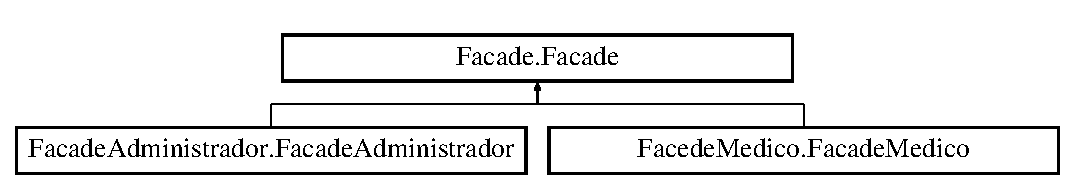
\includegraphics[height=2.000000cm]{class_facade_1_1_facade}
\end{center}
\end{figure}
\subsection*{Public Member Functions}
\begin{DoxyCompactItemize}
\item 
def \mbox{\hyperlink{class_facade_1_1_facade_ad3ab1700c8824f9711bb33c34187f2b4}{\+\_\+\+\_\+init\+\_\+\+\_\+}} (self)
\item 
def \mbox{\hyperlink{class_facade_1_1_facade_ab29afbe3462ddbb2e6d8203d20f610ae}{cargar\+\_\+imagen}} (self, nombre)
\begin{DoxyCompactList}\small\item\em Documentation Cargar imagen. \end{DoxyCompactList}\item 
def \mbox{\hyperlink{class_facade_1_1_facade_a31c82e317bb43cffa46140c2826a908b}{estimar\+\_\+edad}} (self)
\begin{DoxyCompactList}\small\item\em Documentation estimar\+\_\+edad. \end{DoxyCompactList}\item 
def \mbox{\hyperlink{class_facade_1_1_facade_a92d3a050a1526997ed8d0c080c016b77}{desplegar\+\_\+edad}} (self)
\begin{DoxyCompactList}\small\item\em Documentation desplegar\+\_\+edad. \end{DoxyCompactList}\item 
def \mbox{\hyperlink{class_facade_1_1_facade_a1bf0fe7872a81826af422d1efeccef92}{guardar\+\_\+informacion\+\_\+paciente}} (self, datos)
\begin{DoxyCompactList}\small\item\em Documentation guardar\+\_\+informacion\+\_\+paciente. \end{DoxyCompactList}\item 
def \mbox{\hyperlink{class_facade_1_1_facade_a1771449006d9324bae3c3449f59b8fe6}{cargar\+\_\+imagenes}} (self, direccion)
\begin{DoxyCompactList}\small\item\em Documentation Cargar\+\_\+imagenes. \end{DoxyCompactList}\item 
def \mbox{\hyperlink{class_facade_1_1_facade_ad01d3a1108a539ada2d0615c53b160de}{cargar\+\_\+cvs}} (self, nombre)
\begin{DoxyCompactList}\small\item\em Documentation Cargar\+\_\+cvs. \end{DoxyCompactList}\item 
def \mbox{\hyperlink{class_facade_1_1_facade_abb62f6ed9e166bc1041ad7a3c57c4d58}{calcular\+\_\+\+M\+AE}} (self)
\begin{DoxyCompactList}\small\item\em Documentation clacular\+\_\+\+M\+AE. \end{DoxyCompactList}\item 
def \mbox{\hyperlink{class_facade_1_1_facade_a37747590f3e1ade1250e56dd9c424d03}{calcular\+\_\+\+M\+SE}} (self)
\begin{DoxyCompactList}\small\item\em Documentation Calcuar\+\_\+\+M\+SE . \end{DoxyCompactList}\end{DoxyCompactItemize}
\subsection*{Public Attributes}
\begin{DoxyCompactItemize}
\item 
\mbox{\hyperlink{class_facade_1_1_facade_a4ec08f6f7094ff267875a3abc6f0cb1b}{control}}
\begin{DoxyCompactList}\small\item\em The constructor. \end{DoxyCompactList}\end{DoxyCompactItemize}


\subsection{Detailed Description}
Documentation for a class. 

Clase \mbox{\hyperlink{class_facade_1_1_facade}{Facade}}. 

\subsection{Constructor \& Destructor Documentation}
\mbox{\Hypertarget{class_facade_1_1_facade_ad3ab1700c8824f9711bb33c34187f2b4}\label{class_facade_1_1_facade_ad3ab1700c8824f9711bb33c34187f2b4}} 
\index{Facade\+::\+Facade@{Facade\+::\+Facade}!\+\_\+\+\_\+init\+\_\+\+\_\+@{\+\_\+\+\_\+init\+\_\+\+\_\+}}
\index{\+\_\+\+\_\+init\+\_\+\+\_\+@{\+\_\+\+\_\+init\+\_\+\+\_\+}!Facade\+::\+Facade@{Facade\+::\+Facade}}
\subsubsection{\texorpdfstring{\+\_\+\+\_\+init\+\_\+\+\_\+()}{\_\_init\_\_()}}
{\footnotesize\ttfamily def Facade.\+Facade.\+\_\+\+\_\+init\+\_\+\+\_\+ (\begin{DoxyParamCaption}\item[{}]{self }\end{DoxyParamCaption})}



\subsection{Member Function Documentation}
\mbox{\Hypertarget{class_facade_1_1_facade_abb62f6ed9e166bc1041ad7a3c57c4d58}\label{class_facade_1_1_facade_abb62f6ed9e166bc1041ad7a3c57c4d58}} 
\index{Facade\+::\+Facade@{Facade\+::\+Facade}!calcular\+\_\+\+M\+AE@{calcular\+\_\+\+M\+AE}}
\index{calcular\+\_\+\+M\+AE@{calcular\+\_\+\+M\+AE}!Facade\+::\+Facade@{Facade\+::\+Facade}}
\subsubsection{\texorpdfstring{calcular\+\_\+\+M\+A\+E()}{calcular\_MAE()}}
{\footnotesize\ttfamily def Facade.\+Facade.\+calcular\+\_\+\+M\+AE (\begin{DoxyParamCaption}\item[{}]{self }\end{DoxyParamCaption})}



Documentation clacular\+\_\+\+M\+AE. 


\begin{DoxyParams}{Parameters}
{\em self} & \+: \\
\hline
\end{DoxyParams}
\begin{DoxyReturn}{Returns}
true 
\end{DoxyReturn}
\mbox{\Hypertarget{class_facade_1_1_facade_a37747590f3e1ade1250e56dd9c424d03}\label{class_facade_1_1_facade_a37747590f3e1ade1250e56dd9c424d03}} 
\index{Facade\+::\+Facade@{Facade\+::\+Facade}!calcular\+\_\+\+M\+SE@{calcular\+\_\+\+M\+SE}}
\index{calcular\+\_\+\+M\+SE@{calcular\+\_\+\+M\+SE}!Facade\+::\+Facade@{Facade\+::\+Facade}}
\subsubsection{\texorpdfstring{calcular\+\_\+\+M\+S\+E()}{calcular\_MSE()}}
{\footnotesize\ttfamily def Facade.\+Facade.\+calcular\+\_\+\+M\+SE (\begin{DoxyParamCaption}\item[{}]{self }\end{DoxyParamCaption})}



Documentation Calcuar\+\_\+\+M\+SE . 


\begin{DoxyParams}{Parameters}
{\em self} & \+: \\
\hline
\end{DoxyParams}
\begin{DoxyReturn}{Returns}
true 
\end{DoxyReturn}
\mbox{\Hypertarget{class_facade_1_1_facade_ad01d3a1108a539ada2d0615c53b160de}\label{class_facade_1_1_facade_ad01d3a1108a539ada2d0615c53b160de}} 
\index{Facade\+::\+Facade@{Facade\+::\+Facade}!cargar\+\_\+cvs@{cargar\+\_\+cvs}}
\index{cargar\+\_\+cvs@{cargar\+\_\+cvs}!Facade\+::\+Facade@{Facade\+::\+Facade}}
\subsubsection{\texorpdfstring{cargar\+\_\+cvs()}{cargar\_cvs()}}
{\footnotesize\ttfamily def Facade.\+Facade.\+cargar\+\_\+cvs (\begin{DoxyParamCaption}\item[{}]{self,  }\item[{}]{nombre }\end{DoxyParamCaption})}



Documentation Cargar\+\_\+cvs. 


\begin{DoxyParams}{Parameters}
{\em self} & \+: \\
\hline
{\em nombre} & \+: string \\
\hline
\end{DoxyParams}
\begin{DoxyReturn}{Returns}
true 
\end{DoxyReturn}
\mbox{\Hypertarget{class_facade_1_1_facade_ab29afbe3462ddbb2e6d8203d20f610ae}\label{class_facade_1_1_facade_ab29afbe3462ddbb2e6d8203d20f610ae}} 
\index{Facade\+::\+Facade@{Facade\+::\+Facade}!cargar\+\_\+imagen@{cargar\+\_\+imagen}}
\index{cargar\+\_\+imagen@{cargar\+\_\+imagen}!Facade\+::\+Facade@{Facade\+::\+Facade}}
\subsubsection{\texorpdfstring{cargar\+\_\+imagen()}{cargar\_imagen()}}
{\footnotesize\ttfamily def Facade.\+Facade.\+cargar\+\_\+imagen (\begin{DoxyParamCaption}\item[{}]{self,  }\item[{}]{nombre }\end{DoxyParamCaption})}



Documentation Cargar imagen. 


\begin{DoxyParams}{Parameters}
{\em self} & \+: \\
\hline
{\em nombre} & \+: string ~\newline
 \\
\hline
\end{DoxyParams}
\begin{DoxyReturn}{Returns}
true 
\end{DoxyReturn}
\mbox{\Hypertarget{class_facade_1_1_facade_a1771449006d9324bae3c3449f59b8fe6}\label{class_facade_1_1_facade_a1771449006d9324bae3c3449f59b8fe6}} 
\index{Facade\+::\+Facade@{Facade\+::\+Facade}!cargar\+\_\+imagenes@{cargar\+\_\+imagenes}}
\index{cargar\+\_\+imagenes@{cargar\+\_\+imagenes}!Facade\+::\+Facade@{Facade\+::\+Facade}}
\subsubsection{\texorpdfstring{cargar\+\_\+imagenes()}{cargar\_imagenes()}}
{\footnotesize\ttfamily def Facade.\+Facade.\+cargar\+\_\+imagenes (\begin{DoxyParamCaption}\item[{}]{self,  }\item[{}]{direccion }\end{DoxyParamCaption})}



Documentation Cargar\+\_\+imagenes. 


\begin{DoxyParams}{Parameters}
{\em self} & \+: \\
\hline
{\em direccion} & \+: string \\
\hline
\end{DoxyParams}
\begin{DoxyReturn}{Returns}
true 
\end{DoxyReturn}
\mbox{\Hypertarget{class_facade_1_1_facade_a92d3a050a1526997ed8d0c080c016b77}\label{class_facade_1_1_facade_a92d3a050a1526997ed8d0c080c016b77}} 
\index{Facade\+::\+Facade@{Facade\+::\+Facade}!desplegar\+\_\+edad@{desplegar\+\_\+edad}}
\index{desplegar\+\_\+edad@{desplegar\+\_\+edad}!Facade\+::\+Facade@{Facade\+::\+Facade}}
\subsubsection{\texorpdfstring{desplegar\+\_\+edad()}{desplegar\_edad()}}
{\footnotesize\ttfamily def Facade.\+Facade.\+desplegar\+\_\+edad (\begin{DoxyParamCaption}\item[{}]{self }\end{DoxyParamCaption})}



Documentation desplegar\+\_\+edad. 


\begin{DoxyParams}{Parameters}
{\em self} & \+: \\
\hline
\end{DoxyParams}
\begin{DoxyReturn}{Returns}
true 
\end{DoxyReturn}
\mbox{\Hypertarget{class_facade_1_1_facade_a31c82e317bb43cffa46140c2826a908b}\label{class_facade_1_1_facade_a31c82e317bb43cffa46140c2826a908b}} 
\index{Facade\+::\+Facade@{Facade\+::\+Facade}!estimar\+\_\+edad@{estimar\+\_\+edad}}
\index{estimar\+\_\+edad@{estimar\+\_\+edad}!Facade\+::\+Facade@{Facade\+::\+Facade}}
\subsubsection{\texorpdfstring{estimar\+\_\+edad()}{estimar\_edad()}}
{\footnotesize\ttfamily def Facade.\+Facade.\+estimar\+\_\+edad (\begin{DoxyParamCaption}\item[{}]{self }\end{DoxyParamCaption})}



Documentation estimar\+\_\+edad. 


\begin{DoxyParams}{Parameters}
{\em self} & \+: \\
\hline
\end{DoxyParams}
\begin{DoxyReturn}{Returns}
true 
\end{DoxyReturn}
\mbox{\Hypertarget{class_facade_1_1_facade_a1bf0fe7872a81826af422d1efeccef92}\label{class_facade_1_1_facade_a1bf0fe7872a81826af422d1efeccef92}} 
\index{Facade\+::\+Facade@{Facade\+::\+Facade}!guardar\+\_\+informacion\+\_\+paciente@{guardar\+\_\+informacion\+\_\+paciente}}
\index{guardar\+\_\+informacion\+\_\+paciente@{guardar\+\_\+informacion\+\_\+paciente}!Facade\+::\+Facade@{Facade\+::\+Facade}}
\subsubsection{\texorpdfstring{guardar\+\_\+informacion\+\_\+paciente()}{guardar\_informacion\_paciente()}}
{\footnotesize\ttfamily def Facade.\+Facade.\+guardar\+\_\+informacion\+\_\+paciente (\begin{DoxyParamCaption}\item[{}]{self,  }\item[{}]{datos }\end{DoxyParamCaption})}



Documentation guardar\+\_\+informacion\+\_\+paciente. 


\begin{DoxyParams}{Parameters}
{\em self} & \+: \\
\hline
{\em datos} & \+: \mbox{\hyperlink{namespace_d_t_o_paciente}{D\+T\+O\+Paciente}} \\
\hline
\end{DoxyParams}
\begin{DoxyReturn}{Returns}
true 
\end{DoxyReturn}


\subsection{Member Data Documentation}
\mbox{\Hypertarget{class_facade_1_1_facade_a4ec08f6f7094ff267875a3abc6f0cb1b}\label{class_facade_1_1_facade_a4ec08f6f7094ff267875a3abc6f0cb1b}} 
\index{Facade\+::\+Facade@{Facade\+::\+Facade}!control@{control}}
\index{control@{control}!Facade\+::\+Facade@{Facade\+::\+Facade}}
\subsubsection{\texorpdfstring{control}{control}}
{\footnotesize\ttfamily Facade.\+Facade.\+control}



The constructor. 



The documentation for this class was generated from the following file\+:\begin{DoxyCompactItemize}
\item 
C\+:/\+Users/olman/\+Documents/\+Git\+Hub/\+A\+S\+C-\/\+Proyecto-\/\+I\+S-\/2018/website/main/back\+\_\+end/control/\mbox{\hyperlink{_facade_8py}{Facade.\+py}}\end{DoxyCompactItemize}

\hypertarget{class_facade_administrador_1_1_facade_administrador}{}\section{Facade\+Administrador.\+Facade\+Administrador Class Reference}
\label{class_facade_administrador_1_1_facade_administrador}\index{Facade\+Administrador.\+Facade\+Administrador@{Facade\+Administrador.\+Facade\+Administrador}}


Documentation for a class.  


Inheritance diagram for Facade\+Administrador.\+Facade\+Administrador\+:\begin{figure}[H]
\begin{center}
\leavevmode
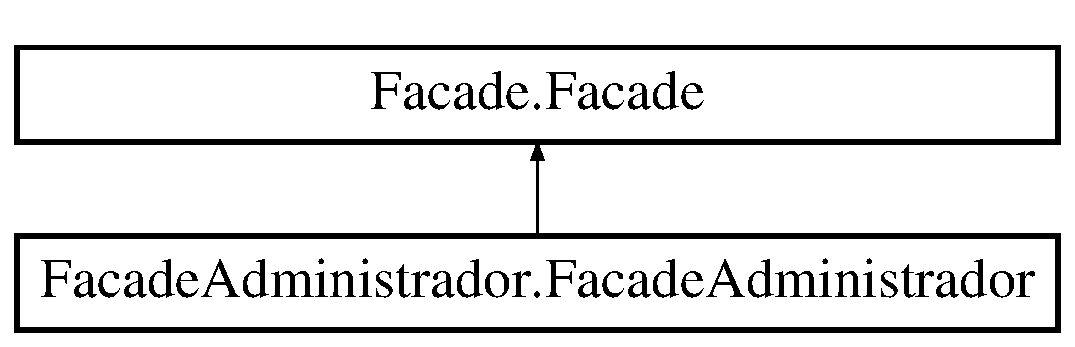
\includegraphics[height=2.000000cm]{class_facade_administrador_1_1_facade_administrador}
\end{center}
\end{figure}
\subsection*{Public Member Functions}
\begin{DoxyCompactItemize}
\item 
def \mbox{\hyperlink{class_facade_administrador_1_1_facade_administrador_aaa6a3941eb11cb692c9ecc712db5af0b}{\+\_\+\+\_\+init\+\_\+\+\_\+}} (self)
\item 
def \mbox{\hyperlink{class_facade_administrador_1_1_facade_administrador_aca7528cedb162799ab858010207a5dab}{cargar\+\_\+imagenes}} (self, direccion)
\begin{DoxyCompactList}\small\item\em Documentation Cargar imagenes. \end{DoxyCompactList}\item 
def \mbox{\hyperlink{class_facade_administrador_1_1_facade_administrador_aaf2e6dac8063826680c1ae5a62314e2f}{cargar\+\_\+cvs}} (self, nombre)
\begin{DoxyCompactList}\small\item\em Documentation Cargar\+\_\+cvs. \end{DoxyCompactList}\item 
def \mbox{\hyperlink{class_facade_administrador_1_1_facade_administrador_ac65ea555d12893eb9ce5a1ec20c31165}{calcular\+\_\+\+M\+AE}} (self)
\begin{DoxyCompactList}\small\item\em Documentation clacular\+\_\+\+M\+AE. \end{DoxyCompactList}\item 
def \mbox{\hyperlink{class_facade_administrador_1_1_facade_administrador_a06b10fce3e70d4292f4c2fae5026643c}{calcular\+\_\+\+M\+SE}} (self)
\begin{DoxyCompactList}\small\item\em Documentation clacular\+\_\+\+M\+SE. \end{DoxyCompactList}\end{DoxyCompactItemize}
\subsection*{Additional Inherited Members}


\subsection{Detailed Description}
Documentation for a class. 

Clase \mbox{\hyperlink{class_facade_administrador_1_1_facade_administrador}{Facade\+Administrador}}. 

\subsection{Constructor \& Destructor Documentation}
\mbox{\Hypertarget{class_facade_administrador_1_1_facade_administrador_aaa6a3941eb11cb692c9ecc712db5af0b}\label{class_facade_administrador_1_1_facade_administrador_aaa6a3941eb11cb692c9ecc712db5af0b}} 
\index{Facade\+Administrador\+::\+Facade\+Administrador@{Facade\+Administrador\+::\+Facade\+Administrador}!\+\_\+\+\_\+init\+\_\+\+\_\+@{\+\_\+\+\_\+init\+\_\+\+\_\+}}
\index{\+\_\+\+\_\+init\+\_\+\+\_\+@{\+\_\+\+\_\+init\+\_\+\+\_\+}!Facade\+Administrador\+::\+Facade\+Administrador@{Facade\+Administrador\+::\+Facade\+Administrador}}
\subsubsection{\texorpdfstring{\+\_\+\+\_\+init\+\_\+\+\_\+()}{\_\_init\_\_()}}
{\footnotesize\ttfamily def Facade\+Administrador.\+Facade\+Administrador.\+\_\+\+\_\+init\+\_\+\+\_\+ (\begin{DoxyParamCaption}\item[{}]{self }\end{DoxyParamCaption})}



\subsection{Member Function Documentation}
\mbox{\Hypertarget{class_facade_administrador_1_1_facade_administrador_ac65ea555d12893eb9ce5a1ec20c31165}\label{class_facade_administrador_1_1_facade_administrador_ac65ea555d12893eb9ce5a1ec20c31165}} 
\index{Facade\+Administrador\+::\+Facade\+Administrador@{Facade\+Administrador\+::\+Facade\+Administrador}!calcular\+\_\+\+M\+AE@{calcular\+\_\+\+M\+AE}}
\index{calcular\+\_\+\+M\+AE@{calcular\+\_\+\+M\+AE}!Facade\+Administrador\+::\+Facade\+Administrador@{Facade\+Administrador\+::\+Facade\+Administrador}}
\subsubsection{\texorpdfstring{calcular\+\_\+\+M\+A\+E()}{calcular\_MAE()}}
{\footnotesize\ttfamily def Facade\+Administrador.\+Facade\+Administrador.\+calcular\+\_\+\+M\+AE (\begin{DoxyParamCaption}\item[{}]{self }\end{DoxyParamCaption})}



Documentation clacular\+\_\+\+M\+AE. 


\begin{DoxyParams}{Parameters}
{\em self} & \+: \\
\hline
\end{DoxyParams}
\begin{DoxyReturn}{Returns}
true 
\end{DoxyReturn}
\mbox{\Hypertarget{class_facade_administrador_1_1_facade_administrador_a06b10fce3e70d4292f4c2fae5026643c}\label{class_facade_administrador_1_1_facade_administrador_a06b10fce3e70d4292f4c2fae5026643c}} 
\index{Facade\+Administrador\+::\+Facade\+Administrador@{Facade\+Administrador\+::\+Facade\+Administrador}!calcular\+\_\+\+M\+SE@{calcular\+\_\+\+M\+SE}}
\index{calcular\+\_\+\+M\+SE@{calcular\+\_\+\+M\+SE}!Facade\+Administrador\+::\+Facade\+Administrador@{Facade\+Administrador\+::\+Facade\+Administrador}}
\subsubsection{\texorpdfstring{calcular\+\_\+\+M\+S\+E()}{calcular\_MSE()}}
{\footnotesize\ttfamily def Facade\+Administrador.\+Facade\+Administrador.\+calcular\+\_\+\+M\+SE (\begin{DoxyParamCaption}\item[{}]{self }\end{DoxyParamCaption})}



Documentation clacular\+\_\+\+M\+SE. 


\begin{DoxyParams}{Parameters}
{\em self} & \+: \\
\hline
\end{DoxyParams}
\begin{DoxyReturn}{Returns}
true 
\end{DoxyReturn}
\mbox{\Hypertarget{class_facade_administrador_1_1_facade_administrador_aaf2e6dac8063826680c1ae5a62314e2f}\label{class_facade_administrador_1_1_facade_administrador_aaf2e6dac8063826680c1ae5a62314e2f}} 
\index{Facade\+Administrador\+::\+Facade\+Administrador@{Facade\+Administrador\+::\+Facade\+Administrador}!cargar\+\_\+cvs@{cargar\+\_\+cvs}}
\index{cargar\+\_\+cvs@{cargar\+\_\+cvs}!Facade\+Administrador\+::\+Facade\+Administrador@{Facade\+Administrador\+::\+Facade\+Administrador}}
\subsubsection{\texorpdfstring{cargar\+\_\+cvs()}{cargar\_cvs()}}
{\footnotesize\ttfamily def Facade\+Administrador.\+Facade\+Administrador.\+cargar\+\_\+cvs (\begin{DoxyParamCaption}\item[{}]{self,  }\item[{}]{nombre }\end{DoxyParamCaption})}



Documentation Cargar\+\_\+cvs. 


\begin{DoxyParams}{Parameters}
{\em self} & \+: \\
\hline
{\em nombre} & \+: string \\
\hline
\end{DoxyParams}
\begin{DoxyReturn}{Returns}
true 
\end{DoxyReturn}
\mbox{\Hypertarget{class_facade_administrador_1_1_facade_administrador_aca7528cedb162799ab858010207a5dab}\label{class_facade_administrador_1_1_facade_administrador_aca7528cedb162799ab858010207a5dab}} 
\index{Facade\+Administrador\+::\+Facade\+Administrador@{Facade\+Administrador\+::\+Facade\+Administrador}!cargar\+\_\+imagenes@{cargar\+\_\+imagenes}}
\index{cargar\+\_\+imagenes@{cargar\+\_\+imagenes}!Facade\+Administrador\+::\+Facade\+Administrador@{Facade\+Administrador\+::\+Facade\+Administrador}}
\subsubsection{\texorpdfstring{cargar\+\_\+imagenes()}{cargar\_imagenes()}}
{\footnotesize\ttfamily def Facade\+Administrador.\+Facade\+Administrador.\+cargar\+\_\+imagenes (\begin{DoxyParamCaption}\item[{}]{self,  }\item[{}]{direccion }\end{DoxyParamCaption})}



Documentation Cargar imagenes. 


\begin{DoxyParams}{Parameters}
{\em self} & \+: \\
\hline
{\em direccion} & \+: string \\
\hline
\end{DoxyParams}
\begin{DoxyReturn}{Returns}
true 
\end{DoxyReturn}


The documentation for this class was generated from the following file\+:\begin{DoxyCompactItemize}
\item 
C\+:/\+Users/olman/\+Documents/\+Git\+Hub/\+A\+S\+C-\/\+Proyecto-\/\+I\+S-\/2018/website/main/back\+\_\+end/control/\mbox{\hyperlink{_facade_administrador_8py}{Facade\+Administrador.\+py}}\end{DoxyCompactItemize}

\hypertarget{class_facede_medico_1_1_facade_medico}{}\section{Facede\+Medico.\+Facade\+Medico Class Reference}
\label{class_facede_medico_1_1_facade_medico}\index{Facede\+Medico.\+Facade\+Medico@{Facede\+Medico.\+Facade\+Medico}}
Inheritance diagram for Facede\+Medico.\+Facade\+Medico\+:\begin{figure}[H]
\begin{center}
\leavevmode
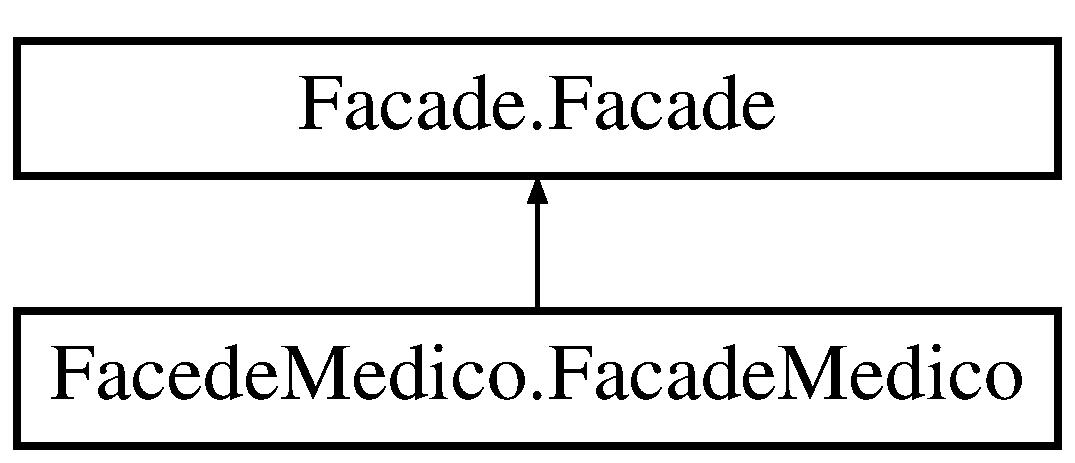
\includegraphics[height=2.000000cm]{class_facede_medico_1_1_facade_medico}
\end{center}
\end{figure}
\subsection*{Public Member Functions}
\begin{DoxyCompactItemize}
\item 
def \mbox{\hyperlink{class_facede_medico_1_1_facade_medico_a461dbe3bea34efedec3c2425e48982da}{\+\_\+\+\_\+init\+\_\+\+\_\+}} (self)
\item 
def \mbox{\hyperlink{class_facede_medico_1_1_facade_medico_a2d0ba068aaf9eaa04d9b297ed947e9c7}{cargar\+\_\+imagen}} (self)
\item 
def \mbox{\hyperlink{class_facede_medico_1_1_facade_medico_a23738769ea9bd5016e9bc191c83a3fed}{estimar\+\_\+edad}} (self)
\item 
def \mbox{\hyperlink{class_facede_medico_1_1_facade_medico_a865f5e402914ba2461306bed197fc3c7}{desplegar\+\_\+edad}} (self)
\item 
def \mbox{\hyperlink{class_facede_medico_1_1_facade_medico_a4acf15afa074658561ab423294821c74}{guardar\+\_\+informacion\+\_\+paciente}} (self)
\end{DoxyCompactItemize}
\subsection*{Additional Inherited Members}


\subsection{Constructor \& Destructor Documentation}
\mbox{\Hypertarget{class_facede_medico_1_1_facade_medico_a461dbe3bea34efedec3c2425e48982da}\label{class_facede_medico_1_1_facade_medico_a461dbe3bea34efedec3c2425e48982da}} 
\index{Facede\+Medico\+::\+Facade\+Medico@{Facede\+Medico\+::\+Facade\+Medico}!\+\_\+\+\_\+init\+\_\+\+\_\+@{\+\_\+\+\_\+init\+\_\+\+\_\+}}
\index{\+\_\+\+\_\+init\+\_\+\+\_\+@{\+\_\+\+\_\+init\+\_\+\+\_\+}!Facede\+Medico\+::\+Facade\+Medico@{Facede\+Medico\+::\+Facade\+Medico}}
\subsubsection{\texorpdfstring{\+\_\+\+\_\+init\+\_\+\+\_\+()}{\_\_init\_\_()}}
{\footnotesize\ttfamily def Facede\+Medico.\+Facade\+Medico.\+\_\+\+\_\+init\+\_\+\+\_\+ (\begin{DoxyParamCaption}\item[{}]{self }\end{DoxyParamCaption})}



\subsection{Member Function Documentation}
\mbox{\Hypertarget{class_facede_medico_1_1_facade_medico_a2d0ba068aaf9eaa04d9b297ed947e9c7}\label{class_facede_medico_1_1_facade_medico_a2d0ba068aaf9eaa04d9b297ed947e9c7}} 
\index{Facede\+Medico\+::\+Facade\+Medico@{Facede\+Medico\+::\+Facade\+Medico}!cargar\+\_\+imagen@{cargar\+\_\+imagen}}
\index{cargar\+\_\+imagen@{cargar\+\_\+imagen}!Facede\+Medico\+::\+Facade\+Medico@{Facede\+Medico\+::\+Facade\+Medico}}
\subsubsection{\texorpdfstring{cargar\+\_\+imagen()}{cargar\_imagen()}}
{\footnotesize\ttfamily def Facede\+Medico.\+Facade\+Medico.\+cargar\+\_\+imagen (\begin{DoxyParamCaption}\item[{}]{self }\end{DoxyParamCaption})}

\mbox{\Hypertarget{class_facede_medico_1_1_facade_medico_a865f5e402914ba2461306bed197fc3c7}\label{class_facede_medico_1_1_facade_medico_a865f5e402914ba2461306bed197fc3c7}} 
\index{Facede\+Medico\+::\+Facade\+Medico@{Facede\+Medico\+::\+Facade\+Medico}!desplegar\+\_\+edad@{desplegar\+\_\+edad}}
\index{desplegar\+\_\+edad@{desplegar\+\_\+edad}!Facede\+Medico\+::\+Facade\+Medico@{Facede\+Medico\+::\+Facade\+Medico}}
\subsubsection{\texorpdfstring{desplegar\+\_\+edad()}{desplegar\_edad()}}
{\footnotesize\ttfamily def Facede\+Medico.\+Facade\+Medico.\+desplegar\+\_\+edad (\begin{DoxyParamCaption}\item[{}]{self }\end{DoxyParamCaption})}

\mbox{\Hypertarget{class_facede_medico_1_1_facade_medico_a23738769ea9bd5016e9bc191c83a3fed}\label{class_facede_medico_1_1_facade_medico_a23738769ea9bd5016e9bc191c83a3fed}} 
\index{Facede\+Medico\+::\+Facade\+Medico@{Facede\+Medico\+::\+Facade\+Medico}!estimar\+\_\+edad@{estimar\+\_\+edad}}
\index{estimar\+\_\+edad@{estimar\+\_\+edad}!Facede\+Medico\+::\+Facade\+Medico@{Facede\+Medico\+::\+Facade\+Medico}}
\subsubsection{\texorpdfstring{estimar\+\_\+edad()}{estimar\_edad()}}
{\footnotesize\ttfamily def Facede\+Medico.\+Facade\+Medico.\+estimar\+\_\+edad (\begin{DoxyParamCaption}\item[{}]{self }\end{DoxyParamCaption})}

\mbox{\Hypertarget{class_facede_medico_1_1_facade_medico_a4acf15afa074658561ab423294821c74}\label{class_facede_medico_1_1_facade_medico_a4acf15afa074658561ab423294821c74}} 
\index{Facede\+Medico\+::\+Facade\+Medico@{Facede\+Medico\+::\+Facade\+Medico}!guardar\+\_\+informacion\+\_\+paciente@{guardar\+\_\+informacion\+\_\+paciente}}
\index{guardar\+\_\+informacion\+\_\+paciente@{guardar\+\_\+informacion\+\_\+paciente}!Facede\+Medico\+::\+Facade\+Medico@{Facede\+Medico\+::\+Facade\+Medico}}
\subsubsection{\texorpdfstring{guardar\+\_\+informacion\+\_\+paciente()}{guardar\_informacion\_paciente()}}
{\footnotesize\ttfamily def Facede\+Medico.\+Facade\+Medico.\+guardar\+\_\+informacion\+\_\+paciente (\begin{DoxyParamCaption}\item[{}]{self }\end{DoxyParamCaption})}



The documentation for this class was generated from the following file\+:\begin{DoxyCompactItemize}
\item 
control/\mbox{\hyperlink{_facede_medico_8py}{Facede\+Medico.\+py}}\end{DoxyCompactItemize}

\hypertarget{class_gestor_muestra_1_1_gestor_muestra}{}\section{Gestor\+Muestra.\+Gestor\+Muestra Class Reference}
\label{class_gestor_muestra_1_1_gestor_muestra}\index{Gestor\+Muestra.\+Gestor\+Muestra@{Gestor\+Muestra.\+Gestor\+Muestra}}
\subsection*{Public Member Functions}
\begin{DoxyCompactItemize}
\item 
def \mbox{\hyperlink{class_gestor_muestra_1_1_gestor_muestra_a4ecb9256f16f15aa652b277297eb8879}{\+\_\+\+\_\+init\+\_\+\+\_\+}} (self)
\item 
def \mbox{\hyperlink{class_gestor_muestra_1_1_gestor_muestra_a3acc1dd10c8408638d2079a22a4ce373}{cargar\+\_\+imagenes}} (self)
\item 
def \mbox{\hyperlink{class_gestor_muestra_1_1_gestor_muestra_ab63f7733704d3f96d3c35f36481b3c21}{cargar\+\_\+cvs}} (self)
\end{DoxyCompactItemize}
\subsection*{Public Attributes}
\begin{DoxyCompactItemize}
\item 
\mbox{\hyperlink{class_gestor_muestra_1_1_gestor_muestra_ab4df90a4af99c2d10b6b1d468d45f7d7}{DB}}
\end{DoxyCompactItemize}


\subsection{Constructor \& Destructor Documentation}
\mbox{\Hypertarget{class_gestor_muestra_1_1_gestor_muestra_a4ecb9256f16f15aa652b277297eb8879}\label{class_gestor_muestra_1_1_gestor_muestra_a4ecb9256f16f15aa652b277297eb8879}} 
\index{Gestor\+Muestra\+::\+Gestor\+Muestra@{Gestor\+Muestra\+::\+Gestor\+Muestra}!\+\_\+\+\_\+init\+\_\+\+\_\+@{\+\_\+\+\_\+init\+\_\+\+\_\+}}
\index{\+\_\+\+\_\+init\+\_\+\+\_\+@{\+\_\+\+\_\+init\+\_\+\+\_\+}!Gestor\+Muestra\+::\+Gestor\+Muestra@{Gestor\+Muestra\+::\+Gestor\+Muestra}}
\subsubsection{\texorpdfstring{\+\_\+\+\_\+init\+\_\+\+\_\+()}{\_\_init\_\_()}}
{\footnotesize\ttfamily def Gestor\+Muestra.\+Gestor\+Muestra.\+\_\+\+\_\+init\+\_\+\+\_\+ (\begin{DoxyParamCaption}\item[{}]{self }\end{DoxyParamCaption})}



\subsection{Member Function Documentation}
\mbox{\Hypertarget{class_gestor_muestra_1_1_gestor_muestra_ab63f7733704d3f96d3c35f36481b3c21}\label{class_gestor_muestra_1_1_gestor_muestra_ab63f7733704d3f96d3c35f36481b3c21}} 
\index{Gestor\+Muestra\+::\+Gestor\+Muestra@{Gestor\+Muestra\+::\+Gestor\+Muestra}!cargar\+\_\+cvs@{cargar\+\_\+cvs}}
\index{cargar\+\_\+cvs@{cargar\+\_\+cvs}!Gestor\+Muestra\+::\+Gestor\+Muestra@{Gestor\+Muestra\+::\+Gestor\+Muestra}}
\subsubsection{\texorpdfstring{cargar\+\_\+cvs()}{cargar\_cvs()}}
{\footnotesize\ttfamily def Gestor\+Muestra.\+Gestor\+Muestra.\+cargar\+\_\+cvs (\begin{DoxyParamCaption}\item[{}]{self }\end{DoxyParamCaption})}

\mbox{\Hypertarget{class_gestor_muestra_1_1_gestor_muestra_a3acc1dd10c8408638d2079a22a4ce373}\label{class_gestor_muestra_1_1_gestor_muestra_a3acc1dd10c8408638d2079a22a4ce373}} 
\index{Gestor\+Muestra\+::\+Gestor\+Muestra@{Gestor\+Muestra\+::\+Gestor\+Muestra}!cargar\+\_\+imagenes@{cargar\+\_\+imagenes}}
\index{cargar\+\_\+imagenes@{cargar\+\_\+imagenes}!Gestor\+Muestra\+::\+Gestor\+Muestra@{Gestor\+Muestra\+::\+Gestor\+Muestra}}
\subsubsection{\texorpdfstring{cargar\+\_\+imagenes()}{cargar\_imagenes()}}
{\footnotesize\ttfamily def Gestor\+Muestra.\+Gestor\+Muestra.\+cargar\+\_\+imagenes (\begin{DoxyParamCaption}\item[{}]{self }\end{DoxyParamCaption})}



\subsection{Member Data Documentation}
\mbox{\Hypertarget{class_gestor_muestra_1_1_gestor_muestra_ab4df90a4af99c2d10b6b1d468d45f7d7}\label{class_gestor_muestra_1_1_gestor_muestra_ab4df90a4af99c2d10b6b1d468d45f7d7}} 
\index{Gestor\+Muestra\+::\+Gestor\+Muestra@{Gestor\+Muestra\+::\+Gestor\+Muestra}!DB@{DB}}
\index{DB@{DB}!Gestor\+Muestra\+::\+Gestor\+Muestra@{Gestor\+Muestra\+::\+Gestor\+Muestra}}
\subsubsection{\texorpdfstring{DB}{DB}}
{\footnotesize\ttfamily Gestor\+Muestra.\+Gestor\+Muestra.\+DB}



The documentation for this class was generated from the following file\+:\begin{DoxyCompactItemize}
\item 
control/\mbox{\hyperlink{_gestor_muestra_8py}{Gestor\+Muestra.\+py}}\end{DoxyCompactItemize}

\hypertarget{class_gestor_paciente_1_1_gestor_paciente}{}\section{Gestor\+Paciente.\+Gestor\+Paciente Class Reference}
\label{class_gestor_paciente_1_1_gestor_paciente}\index{Gestor\+Paciente.\+Gestor\+Paciente@{Gestor\+Paciente.\+Gestor\+Paciente}}
\subsection*{Public Member Functions}
\begin{DoxyCompactItemize}
\item 
def \mbox{\hyperlink{class_gestor_paciente_1_1_gestor_paciente_a2950c017c2b347572c1fb0d203c3d995}{\+\_\+\+\_\+init\+\_\+\+\_\+}} (self)
\item 
def \mbox{\hyperlink{class_gestor_paciente_1_1_gestor_paciente_aa67ac548d627bedc213c3eb39b051bb9}{guardar\+\_\+informacion\+\_\+paciente}} (self, datos)
\end{DoxyCompactItemize}
\subsection*{Public Attributes}
\begin{DoxyCompactItemize}
\item 
\mbox{\hyperlink{class_gestor_paciente_1_1_gestor_paciente_a99f4445d5dc336acbb8df1c8c273a019}{paciente}}
\item 
\mbox{\hyperlink{class_gestor_paciente_1_1_gestor_paciente_af985b307324e1ed89c05c771af5cd30f}{dao\+\_\+db\+\_\+pacinete}}
\end{DoxyCompactItemize}


\subsection{Constructor \& Destructor Documentation}
\mbox{\Hypertarget{class_gestor_paciente_1_1_gestor_paciente_a2950c017c2b347572c1fb0d203c3d995}\label{class_gestor_paciente_1_1_gestor_paciente_a2950c017c2b347572c1fb0d203c3d995}} 
\index{Gestor\+Paciente\+::\+Gestor\+Paciente@{Gestor\+Paciente\+::\+Gestor\+Paciente}!\+\_\+\+\_\+init\+\_\+\+\_\+@{\+\_\+\+\_\+init\+\_\+\+\_\+}}
\index{\+\_\+\+\_\+init\+\_\+\+\_\+@{\+\_\+\+\_\+init\+\_\+\+\_\+}!Gestor\+Paciente\+::\+Gestor\+Paciente@{Gestor\+Paciente\+::\+Gestor\+Paciente}}
\subsubsection{\texorpdfstring{\+\_\+\+\_\+init\+\_\+\+\_\+()}{\_\_init\_\_()}}
{\footnotesize\ttfamily def Gestor\+Paciente.\+Gestor\+Paciente.\+\_\+\+\_\+init\+\_\+\+\_\+ (\begin{DoxyParamCaption}\item[{}]{self }\end{DoxyParamCaption})}



\subsection{Member Function Documentation}
\mbox{\Hypertarget{class_gestor_paciente_1_1_gestor_paciente_aa67ac548d627bedc213c3eb39b051bb9}\label{class_gestor_paciente_1_1_gestor_paciente_aa67ac548d627bedc213c3eb39b051bb9}} 
\index{Gestor\+Paciente\+::\+Gestor\+Paciente@{Gestor\+Paciente\+::\+Gestor\+Paciente}!guardar\+\_\+informacion\+\_\+paciente@{guardar\+\_\+informacion\+\_\+paciente}}
\index{guardar\+\_\+informacion\+\_\+paciente@{guardar\+\_\+informacion\+\_\+paciente}!Gestor\+Paciente\+::\+Gestor\+Paciente@{Gestor\+Paciente\+::\+Gestor\+Paciente}}
\subsubsection{\texorpdfstring{guardar\+\_\+informacion\+\_\+paciente()}{guardar\_informacion\_paciente()}}
{\footnotesize\ttfamily def Gestor\+Paciente.\+Gestor\+Paciente.\+guardar\+\_\+informacion\+\_\+paciente (\begin{DoxyParamCaption}\item[{}]{self,  }\item[{}]{datos }\end{DoxyParamCaption})}



\subsection{Member Data Documentation}
\mbox{\Hypertarget{class_gestor_paciente_1_1_gestor_paciente_af985b307324e1ed89c05c771af5cd30f}\label{class_gestor_paciente_1_1_gestor_paciente_af985b307324e1ed89c05c771af5cd30f}} 
\index{Gestor\+Paciente\+::\+Gestor\+Paciente@{Gestor\+Paciente\+::\+Gestor\+Paciente}!dao\+\_\+db\+\_\+pacinete@{dao\+\_\+db\+\_\+pacinete}}
\index{dao\+\_\+db\+\_\+pacinete@{dao\+\_\+db\+\_\+pacinete}!Gestor\+Paciente\+::\+Gestor\+Paciente@{Gestor\+Paciente\+::\+Gestor\+Paciente}}
\subsubsection{\texorpdfstring{dao\+\_\+db\+\_\+pacinete}{dao\_db\_pacinete}}
{\footnotesize\ttfamily Gestor\+Paciente.\+Gestor\+Paciente.\+dao\+\_\+db\+\_\+pacinete}

\mbox{\Hypertarget{class_gestor_paciente_1_1_gestor_paciente_a99f4445d5dc336acbb8df1c8c273a019}\label{class_gestor_paciente_1_1_gestor_paciente_a99f4445d5dc336acbb8df1c8c273a019}} 
\index{Gestor\+Paciente\+::\+Gestor\+Paciente@{Gestor\+Paciente\+::\+Gestor\+Paciente}!paciente@{paciente}}
\index{paciente@{paciente}!Gestor\+Paciente\+::\+Gestor\+Paciente@{Gestor\+Paciente\+::\+Gestor\+Paciente}}
\subsubsection{\texorpdfstring{paciente}{paciente}}
{\footnotesize\ttfamily Gestor\+Paciente.\+Gestor\+Paciente.\+paciente}



The documentation for this class was generated from the following file\+:\begin{DoxyCompactItemize}
\item 
control/\mbox{\hyperlink{_gestor_paciente_8py}{Gestor\+Paciente.\+py}}\end{DoxyCompactItemize}

\hypertarget{class_imagen_1_1_imagen}{}\section{Imagen.\+Imagen Class Reference}
\label{class_imagen_1_1_imagen}\index{Imagen.\+Imagen@{Imagen.\+Imagen}}


Documentation for a class.  


\subsection*{Public Member Functions}
\begin{DoxyCompactItemize}
\item 
def \mbox{\hyperlink{class_imagen_1_1_imagen_af56feb3348d81937a479c64de374d422}{\+\_\+\+\_\+init\+\_\+\+\_\+}} (self, \mbox{\hyperlink{class_imagen_1_1_imagen_ae3a41e1a6fae0affa3b4735c50212093}{img}}=None)
\item 
def \mbox{\hyperlink{class_imagen_1_1_imagen_a4cdb42ba6cf651b032e66111f2a28219}{vectorizar}} (self)
\begin{DoxyCompactList}\small\item\em Documentation vectorizar. \end{DoxyCompactList}\item 
def \mbox{\hyperlink{class_imagen_1_1_imagen_a76c63b1c129f5ef3e7ea63802209e645}{leer\+\_\+imagen}} (self, directorio)
\begin{DoxyCompactList}\small\item\em Documentation leer\+\_\+imagen. \end{DoxyCompactList}\end{DoxyCompactItemize}
\subsection*{Public Attributes}
\begin{DoxyCompactItemize}
\item 
\mbox{\hyperlink{class_imagen_1_1_imagen_ae3a41e1a6fae0affa3b4735c50212093}{img}}
\begin{DoxyCompactList}\small\item\em The constructor. \end{DoxyCompactList}\item 
\mbox{\hyperlink{class_imagen_1_1_imagen_ad7ff22a9f89ed827ec52d0ccd8934141}{vector}}
\end{DoxyCompactItemize}


\subsection{Detailed Description}
Documentation for a class. 

Clase \mbox{\hyperlink{namespace_gestor_paciente}{Gestor\+Paciente}}. 

\subsection{Constructor \& Destructor Documentation}
\mbox{\Hypertarget{class_imagen_1_1_imagen_af56feb3348d81937a479c64de374d422}\label{class_imagen_1_1_imagen_af56feb3348d81937a479c64de374d422}} 
\index{Imagen\+::\+Imagen@{Imagen\+::\+Imagen}!\+\_\+\+\_\+init\+\_\+\+\_\+@{\+\_\+\+\_\+init\+\_\+\+\_\+}}
\index{\+\_\+\+\_\+init\+\_\+\+\_\+@{\+\_\+\+\_\+init\+\_\+\+\_\+}!Imagen\+::\+Imagen@{Imagen\+::\+Imagen}}
\subsubsection{\texorpdfstring{\+\_\+\+\_\+init\+\_\+\+\_\+()}{\_\_init\_\_()}}
{\footnotesize\ttfamily def Imagen.\+Imagen.\+\_\+\+\_\+init\+\_\+\+\_\+ (\begin{DoxyParamCaption}\item[{}]{self,  }\item[{}]{img = {\ttfamily None} }\end{DoxyParamCaption})}



\subsection{Member Function Documentation}
\mbox{\Hypertarget{class_imagen_1_1_imagen_a76c63b1c129f5ef3e7ea63802209e645}\label{class_imagen_1_1_imagen_a76c63b1c129f5ef3e7ea63802209e645}} 
\index{Imagen\+::\+Imagen@{Imagen\+::\+Imagen}!leer\+\_\+imagen@{leer\+\_\+imagen}}
\index{leer\+\_\+imagen@{leer\+\_\+imagen}!Imagen\+::\+Imagen@{Imagen\+::\+Imagen}}
\subsubsection{\texorpdfstring{leer\+\_\+imagen()}{leer\_imagen()}}
{\footnotesize\ttfamily def Imagen.\+Imagen.\+leer\+\_\+imagen (\begin{DoxyParamCaption}\item[{}]{self,  }\item[{}]{directorio }\end{DoxyParamCaption})}



Documentation leer\+\_\+imagen. 


\begin{DoxyParams}{Parameters}
{\em self} & \+: \\
\hline
{\em self} & \+: directorio \\
\hline
\end{DoxyParams}
\begin{DoxyReturn}{Returns}
true 
\end{DoxyReturn}
\mbox{\Hypertarget{class_imagen_1_1_imagen_a4cdb42ba6cf651b032e66111f2a28219}\label{class_imagen_1_1_imagen_a4cdb42ba6cf651b032e66111f2a28219}} 
\index{Imagen\+::\+Imagen@{Imagen\+::\+Imagen}!vectorizar@{vectorizar}}
\index{vectorizar@{vectorizar}!Imagen\+::\+Imagen@{Imagen\+::\+Imagen}}
\subsubsection{\texorpdfstring{vectorizar()}{vectorizar()}}
{\footnotesize\ttfamily def Imagen.\+Imagen.\+vectorizar (\begin{DoxyParamCaption}\item[{}]{self }\end{DoxyParamCaption})}



Documentation vectorizar. 


\begin{DoxyParams}{Parameters}
{\em self} & \+: \\
\hline
\end{DoxyParams}
\begin{DoxyReturn}{Returns}
true 
\end{DoxyReturn}


\subsection{Member Data Documentation}
\mbox{\Hypertarget{class_imagen_1_1_imagen_ae3a41e1a6fae0affa3b4735c50212093}\label{class_imagen_1_1_imagen_ae3a41e1a6fae0affa3b4735c50212093}} 
\index{Imagen\+::\+Imagen@{Imagen\+::\+Imagen}!img@{img}}
\index{img@{img}!Imagen\+::\+Imagen@{Imagen\+::\+Imagen}}
\subsubsection{\texorpdfstring{img}{img}}
{\footnotesize\ttfamily Imagen.\+Imagen.\+img}



The constructor. 

\mbox{\Hypertarget{class_imagen_1_1_imagen_ad7ff22a9f89ed827ec52d0ccd8934141}\label{class_imagen_1_1_imagen_ad7ff22a9f89ed827ec52d0ccd8934141}} 
\index{Imagen\+::\+Imagen@{Imagen\+::\+Imagen}!vector@{vector}}
\index{vector@{vector}!Imagen\+::\+Imagen@{Imagen\+::\+Imagen}}
\subsubsection{\texorpdfstring{vector}{vector}}
{\footnotesize\ttfamily Imagen.\+Imagen.\+vector}



The documentation for this class was generated from the following file\+:\begin{DoxyCompactItemize}
\item 
C\+:/\+Users/olman/\+Documents/\+Git\+Hub/\+A\+S\+C-\/\+Proyecto-\/\+I\+S-\/2018/website/main/back\+\_\+end/modelo/\mbox{\hyperlink{_imagen_8py}{Imagen.\+py}}\end{DoxyCompactItemize}

\hypertarget{class_m_a_e_1_1_m_a_e}{}\section{M\+A\+E.\+M\+AE Class Reference}
\label{class_m_a_e_1_1_m_a_e}\index{M\+A\+E.\+M\+AE@{M\+A\+E.\+M\+AE}}


Documentation for a class.  


\subsection*{Public Member Functions}
\begin{DoxyCompactItemize}
\item 
def \mbox{\hyperlink{class_m_a_e_1_1_m_a_e_acf334c43862b1112d21fa019c3827bd0}{\+\_\+\+\_\+init\+\_\+\+\_\+}} (self)
\end{DoxyCompactItemize}
\subsection*{Public Attributes}
\begin{DoxyCompactItemize}
\item 
\mbox{\hyperlink{class_m_a_e_1_1_m_a_e_ae516329fc350a56b5a50fe0b922aa6fa}{x}}
\begin{DoxyCompactList}\small\item\em The constructor. \end{DoxyCompactList}\end{DoxyCompactItemize}


\subsection{Detailed Description}
Documentation for a class. 

Clase \mbox{\hyperlink{class_m_a_e_1_1_m_a_e}{M\+AE}} 

\subsection{Constructor \& Destructor Documentation}
\mbox{\Hypertarget{class_m_a_e_1_1_m_a_e_acf334c43862b1112d21fa019c3827bd0}\label{class_m_a_e_1_1_m_a_e_acf334c43862b1112d21fa019c3827bd0}} 
\index{M\+A\+E\+::\+M\+AE@{M\+A\+E\+::\+M\+AE}!\+\_\+\+\_\+init\+\_\+\+\_\+@{\+\_\+\+\_\+init\+\_\+\+\_\+}}
\index{\+\_\+\+\_\+init\+\_\+\+\_\+@{\+\_\+\+\_\+init\+\_\+\+\_\+}!M\+A\+E\+::\+M\+AE@{M\+A\+E\+::\+M\+AE}}
\subsubsection{\texorpdfstring{\+\_\+\+\_\+init\+\_\+\+\_\+()}{\_\_init\_\_()}}
{\footnotesize\ttfamily def M\+A\+E.\+M\+A\+E.\+\_\+\+\_\+init\+\_\+\+\_\+ (\begin{DoxyParamCaption}\item[{}]{self }\end{DoxyParamCaption})}



\subsection{Member Data Documentation}
\mbox{\Hypertarget{class_m_a_e_1_1_m_a_e_ae516329fc350a56b5a50fe0b922aa6fa}\label{class_m_a_e_1_1_m_a_e_ae516329fc350a56b5a50fe0b922aa6fa}} 
\index{M\+A\+E\+::\+M\+AE@{M\+A\+E\+::\+M\+AE}!x@{x}}
\index{x@{x}!M\+A\+E\+::\+M\+AE@{M\+A\+E\+::\+M\+AE}}
\subsubsection{\texorpdfstring{x}{x}}
{\footnotesize\ttfamily M\+A\+E.\+M\+A\+E.\+x}



The constructor. 



The documentation for this class was generated from the following file\+:\begin{DoxyCompactItemize}
\item 
C\+:/\+Users/olman/\+Documents/\+Git\+Hub/\+A\+S\+C-\/\+Proyecto-\/\+I\+S-\/2018/website/main/back\+\_\+end/modelo/\mbox{\hyperlink{_m_a_e_8py}{M\+A\+E.\+py}}\end{DoxyCompactItemize}

\hypertarget{class_m_s_e_1_1_m_s_e}{}\section{M\+S\+E.\+M\+SE Class Reference}
\label{class_m_s_e_1_1_m_s_e}\index{M\+S\+E.\+M\+SE@{M\+S\+E.\+M\+SE}}


Documentation for a class.  


\subsection*{Public Member Functions}
\begin{DoxyCompactItemize}
\item 
def \mbox{\hyperlink{class_m_s_e_1_1_m_s_e_ac2559b4cd1350480bef5c2cbefd0afe6}{\+\_\+\+\_\+init\+\_\+\+\_\+}} (self)
\end{DoxyCompactItemize}
\subsection*{Public Attributes}
\begin{DoxyCompactItemize}
\item 
\mbox{\hyperlink{class_m_s_e_1_1_m_s_e_a3c8a7df08d33bbbdcce9204075542b25}{x}}
\begin{DoxyCompactList}\small\item\em The constructor. \end{DoxyCompactList}\end{DoxyCompactItemize}


\subsection{Detailed Description}
Documentation for a class. 

Clase \mbox{\hyperlink{class_m_s_e_1_1_m_s_e}{M\+SE}} 

\subsection{Constructor \& Destructor Documentation}
\mbox{\Hypertarget{class_m_s_e_1_1_m_s_e_ac2559b4cd1350480bef5c2cbefd0afe6}\label{class_m_s_e_1_1_m_s_e_ac2559b4cd1350480bef5c2cbefd0afe6}} 
\index{M\+S\+E\+::\+M\+SE@{M\+S\+E\+::\+M\+SE}!\+\_\+\+\_\+init\+\_\+\+\_\+@{\+\_\+\+\_\+init\+\_\+\+\_\+}}
\index{\+\_\+\+\_\+init\+\_\+\+\_\+@{\+\_\+\+\_\+init\+\_\+\+\_\+}!M\+S\+E\+::\+M\+SE@{M\+S\+E\+::\+M\+SE}}
\subsubsection{\texorpdfstring{\+\_\+\+\_\+init\+\_\+\+\_\+()}{\_\_init\_\_()}}
{\footnotesize\ttfamily def M\+S\+E.\+M\+S\+E.\+\_\+\+\_\+init\+\_\+\+\_\+ (\begin{DoxyParamCaption}\item[{}]{self }\end{DoxyParamCaption})}



\subsection{Member Data Documentation}
\mbox{\Hypertarget{class_m_s_e_1_1_m_s_e_a3c8a7df08d33bbbdcce9204075542b25}\label{class_m_s_e_1_1_m_s_e_a3c8a7df08d33bbbdcce9204075542b25}} 
\index{M\+S\+E\+::\+M\+SE@{M\+S\+E\+::\+M\+SE}!x@{x}}
\index{x@{x}!M\+S\+E\+::\+M\+SE@{M\+S\+E\+::\+M\+SE}}
\subsubsection{\texorpdfstring{x}{x}}
{\footnotesize\ttfamily M\+S\+E.\+M\+S\+E.\+x}



The constructor. 



The documentation for this class was generated from the following file\+:\begin{DoxyCompactItemize}
\item 
C\+:/\+Users/olman/\+Documents/\+Git\+Hub/\+A\+S\+C-\/\+Proyecto-\/\+I\+S-\/2018/website/main/back\+\_\+end/modelo/\mbox{\hyperlink{_m_s_e_8py}{M\+S\+E.\+py}}\end{DoxyCompactItemize}

\hypertarget{class_muestra_1_1_muestra}{}\section{Muestra.\+Muestra Class Reference}
\label{class_muestra_1_1_muestra}\index{Muestra.\+Muestra@{Muestra.\+Muestra}}
\subsection*{Public Member Functions}
\begin{DoxyCompactItemize}
\item 
def \mbox{\hyperlink{class_muestra_1_1_muestra_a32851be663e08872a32e6a8ace2a3dbc}{\+\_\+\+\_\+init\+\_\+\+\_\+}} (self)
\end{DoxyCompactItemize}
\subsection*{Public Attributes}
\begin{DoxyCompactItemize}
\item 
\mbox{\hyperlink{class_muestra_1_1_muestra_a8332ed8ec72e86e0edbfa22bed6f3828}{pruebas}}
\item 
\mbox{\hyperlink{class_muestra_1_1_muestra_ab0f909db1b6d6ece313843239809a416}{mae}}
\item 
\mbox{\hyperlink{class_muestra_1_1_muestra_aef455f777517629e914cab0adfc2bf90}{mse}}
\item 
\mbox{\hyperlink{class_muestra_1_1_muestra_a128ddbba3c8cb8f8f98ad88d2b8d20fe}{red}}
\end{DoxyCompactItemize}


\subsection{Constructor \& Destructor Documentation}
\mbox{\Hypertarget{class_muestra_1_1_muestra_a32851be663e08872a32e6a8ace2a3dbc}\label{class_muestra_1_1_muestra_a32851be663e08872a32e6a8ace2a3dbc}} 
\index{Muestra\+::\+Muestra@{Muestra\+::\+Muestra}!\+\_\+\+\_\+init\+\_\+\+\_\+@{\+\_\+\+\_\+init\+\_\+\+\_\+}}
\index{\+\_\+\+\_\+init\+\_\+\+\_\+@{\+\_\+\+\_\+init\+\_\+\+\_\+}!Muestra\+::\+Muestra@{Muestra\+::\+Muestra}}
\subsubsection{\texorpdfstring{\+\_\+\+\_\+init\+\_\+\+\_\+()}{\_\_init\_\_()}}
{\footnotesize\ttfamily def Muestra.\+Muestra.\+\_\+\+\_\+init\+\_\+\+\_\+ (\begin{DoxyParamCaption}\item[{}]{self }\end{DoxyParamCaption})}



\subsection{Member Data Documentation}
\mbox{\Hypertarget{class_muestra_1_1_muestra_ab0f909db1b6d6ece313843239809a416}\label{class_muestra_1_1_muestra_ab0f909db1b6d6ece313843239809a416}} 
\index{Muestra\+::\+Muestra@{Muestra\+::\+Muestra}!mae@{mae}}
\index{mae@{mae}!Muestra\+::\+Muestra@{Muestra\+::\+Muestra}}
\subsubsection{\texorpdfstring{mae}{mae}}
{\footnotesize\ttfamily Muestra.\+Muestra.\+mae}

\mbox{\Hypertarget{class_muestra_1_1_muestra_aef455f777517629e914cab0adfc2bf90}\label{class_muestra_1_1_muestra_aef455f777517629e914cab0adfc2bf90}} 
\index{Muestra\+::\+Muestra@{Muestra\+::\+Muestra}!mse@{mse}}
\index{mse@{mse}!Muestra\+::\+Muestra@{Muestra\+::\+Muestra}}
\subsubsection{\texorpdfstring{mse}{mse}}
{\footnotesize\ttfamily Muestra.\+Muestra.\+mse}

\mbox{\Hypertarget{class_muestra_1_1_muestra_a8332ed8ec72e86e0edbfa22bed6f3828}\label{class_muestra_1_1_muestra_a8332ed8ec72e86e0edbfa22bed6f3828}} 
\index{Muestra\+::\+Muestra@{Muestra\+::\+Muestra}!pruebas@{pruebas}}
\index{pruebas@{pruebas}!Muestra\+::\+Muestra@{Muestra\+::\+Muestra}}
\subsubsection{\texorpdfstring{pruebas}{pruebas}}
{\footnotesize\ttfamily Muestra.\+Muestra.\+pruebas}

\mbox{\Hypertarget{class_muestra_1_1_muestra_a128ddbba3c8cb8f8f98ad88d2b8d20fe}\label{class_muestra_1_1_muestra_a128ddbba3c8cb8f8f98ad88d2b8d20fe}} 
\index{Muestra\+::\+Muestra@{Muestra\+::\+Muestra}!red@{red}}
\index{red@{red}!Muestra\+::\+Muestra@{Muestra\+::\+Muestra}}
\subsubsection{\texorpdfstring{red}{red}}
{\footnotesize\ttfamily Muestra.\+Muestra.\+red}



The documentation for this class was generated from the following file\+:\begin{DoxyCompactItemize}
\item 
modelo/\mbox{\hyperlink{_muestra_8py}{Muestra.\+py}}\end{DoxyCompactItemize}

\hypertarget{class_paciente_1_1_paciente}{}\section{Paciente.\+Paciente Class Reference}
\label{class_paciente_1_1_paciente}\index{Paciente.\+Paciente@{Paciente.\+Paciente}}
\subsection*{Public Member Functions}
\begin{DoxyCompactItemize}
\item 
def \mbox{\hyperlink{class_paciente_1_1_paciente_a2c88db03c95c828f1d0f58e9d32ea355}{\+\_\+\+\_\+init\+\_\+\+\_\+}} (self)
\end{DoxyCompactItemize}
\subsection*{Public Attributes}
\begin{DoxyCompactItemize}
\item 
\mbox{\hyperlink{class_paciente_1_1_paciente_abf70fff36082e22e22c2235768375de3}{edad}}
\item 
\mbox{\hyperlink{class_paciente_1_1_paciente_af256a15938714b75d23283e3ff8fad02}{estimacion\+\_\+edad}}
\item 
\mbox{\hyperlink{class_paciente_1_1_paciente_a5af3b0cc2e0a1469d603f2efea44df45}{url\+\_\+imagen}}
\item 
\mbox{\hyperlink{class_paciente_1_1_paciente_a0df4d67d7a1e91c7cc72b14ca7bd7b78}{nombre}}
\item 
\mbox{\hyperlink{class_paciente_1_1_paciente_a5b4864356ffb572e967ac84c8f1ef563}{apellido\+\_\+1}}
\item 
\mbox{\hyperlink{class_paciente_1_1_paciente_aa6013db207c8415f9878c0a292ab954d}{apellido\+\_\+2}}
\item 
\mbox{\hyperlink{class_paciente_1_1_paciente_ad98665ddc10fc8bc5ff0b6a43ee726f1}{cedula}}
\item 
\mbox{\hyperlink{class_paciente_1_1_paciente_a0c4e9e5166be854ff5dad10248fdb85c}{hospital}}
\item 
\mbox{\hyperlink{class_paciente_1_1_paciente_a2dd715404933b0c95678e27418e139f7}{img}}
\item 
\mbox{\hyperlink{class_paciente_1_1_paciente_ad5dd0b61b2f837ec4f5407ee2a5bb605}{red}}
\end{DoxyCompactItemize}


\subsection{Constructor \& Destructor Documentation}
\mbox{\Hypertarget{class_paciente_1_1_paciente_a2c88db03c95c828f1d0f58e9d32ea355}\label{class_paciente_1_1_paciente_a2c88db03c95c828f1d0f58e9d32ea355}} 
\index{Paciente\+::\+Paciente@{Paciente\+::\+Paciente}!\+\_\+\+\_\+init\+\_\+\+\_\+@{\+\_\+\+\_\+init\+\_\+\+\_\+}}
\index{\+\_\+\+\_\+init\+\_\+\+\_\+@{\+\_\+\+\_\+init\+\_\+\+\_\+}!Paciente\+::\+Paciente@{Paciente\+::\+Paciente}}
\subsubsection{\texorpdfstring{\+\_\+\+\_\+init\+\_\+\+\_\+()}{\_\_init\_\_()}}
{\footnotesize\ttfamily def Paciente.\+Paciente.\+\_\+\+\_\+init\+\_\+\+\_\+ (\begin{DoxyParamCaption}\item[{}]{self }\end{DoxyParamCaption})}



\subsection{Member Data Documentation}
\mbox{\Hypertarget{class_paciente_1_1_paciente_a5b4864356ffb572e967ac84c8f1ef563}\label{class_paciente_1_1_paciente_a5b4864356ffb572e967ac84c8f1ef563}} 
\index{Paciente\+::\+Paciente@{Paciente\+::\+Paciente}!apellido\+\_\+1@{apellido\+\_\+1}}
\index{apellido\+\_\+1@{apellido\+\_\+1}!Paciente\+::\+Paciente@{Paciente\+::\+Paciente}}
\subsubsection{\texorpdfstring{apellido\+\_\+1}{apellido\_1}}
{\footnotesize\ttfamily Paciente.\+Paciente.\+apellido\+\_\+1}

\mbox{\Hypertarget{class_paciente_1_1_paciente_aa6013db207c8415f9878c0a292ab954d}\label{class_paciente_1_1_paciente_aa6013db207c8415f9878c0a292ab954d}} 
\index{Paciente\+::\+Paciente@{Paciente\+::\+Paciente}!apellido\+\_\+2@{apellido\+\_\+2}}
\index{apellido\+\_\+2@{apellido\+\_\+2}!Paciente\+::\+Paciente@{Paciente\+::\+Paciente}}
\subsubsection{\texorpdfstring{apellido\+\_\+2}{apellido\_2}}
{\footnotesize\ttfamily Paciente.\+Paciente.\+apellido\+\_\+2}

\mbox{\Hypertarget{class_paciente_1_1_paciente_ad98665ddc10fc8bc5ff0b6a43ee726f1}\label{class_paciente_1_1_paciente_ad98665ddc10fc8bc5ff0b6a43ee726f1}} 
\index{Paciente\+::\+Paciente@{Paciente\+::\+Paciente}!cedula@{cedula}}
\index{cedula@{cedula}!Paciente\+::\+Paciente@{Paciente\+::\+Paciente}}
\subsubsection{\texorpdfstring{cedula}{cedula}}
{\footnotesize\ttfamily Paciente.\+Paciente.\+cedula}

\mbox{\Hypertarget{class_paciente_1_1_paciente_abf70fff36082e22e22c2235768375de3}\label{class_paciente_1_1_paciente_abf70fff36082e22e22c2235768375de3}} 
\index{Paciente\+::\+Paciente@{Paciente\+::\+Paciente}!edad@{edad}}
\index{edad@{edad}!Paciente\+::\+Paciente@{Paciente\+::\+Paciente}}
\subsubsection{\texorpdfstring{edad}{edad}}
{\footnotesize\ttfamily Paciente.\+Paciente.\+edad}

\mbox{\Hypertarget{class_paciente_1_1_paciente_af256a15938714b75d23283e3ff8fad02}\label{class_paciente_1_1_paciente_af256a15938714b75d23283e3ff8fad02}} 
\index{Paciente\+::\+Paciente@{Paciente\+::\+Paciente}!estimacion\+\_\+edad@{estimacion\+\_\+edad}}
\index{estimacion\+\_\+edad@{estimacion\+\_\+edad}!Paciente\+::\+Paciente@{Paciente\+::\+Paciente}}
\subsubsection{\texorpdfstring{estimacion\+\_\+edad}{estimacion\_edad}}
{\footnotesize\ttfamily Paciente.\+Paciente.\+estimacion\+\_\+edad}

\mbox{\Hypertarget{class_paciente_1_1_paciente_a0c4e9e5166be854ff5dad10248fdb85c}\label{class_paciente_1_1_paciente_a0c4e9e5166be854ff5dad10248fdb85c}} 
\index{Paciente\+::\+Paciente@{Paciente\+::\+Paciente}!hospital@{hospital}}
\index{hospital@{hospital}!Paciente\+::\+Paciente@{Paciente\+::\+Paciente}}
\subsubsection{\texorpdfstring{hospital}{hospital}}
{\footnotesize\ttfamily Paciente.\+Paciente.\+hospital}

\mbox{\Hypertarget{class_paciente_1_1_paciente_a2dd715404933b0c95678e27418e139f7}\label{class_paciente_1_1_paciente_a2dd715404933b0c95678e27418e139f7}} 
\index{Paciente\+::\+Paciente@{Paciente\+::\+Paciente}!img@{img}}
\index{img@{img}!Paciente\+::\+Paciente@{Paciente\+::\+Paciente}}
\subsubsection{\texorpdfstring{img}{img}}
{\footnotesize\ttfamily Paciente.\+Paciente.\+img}

\mbox{\Hypertarget{class_paciente_1_1_paciente_a0df4d67d7a1e91c7cc72b14ca7bd7b78}\label{class_paciente_1_1_paciente_a0df4d67d7a1e91c7cc72b14ca7bd7b78}} 
\index{Paciente\+::\+Paciente@{Paciente\+::\+Paciente}!nombre@{nombre}}
\index{nombre@{nombre}!Paciente\+::\+Paciente@{Paciente\+::\+Paciente}}
\subsubsection{\texorpdfstring{nombre}{nombre}}
{\footnotesize\ttfamily Paciente.\+Paciente.\+nombre}

\mbox{\Hypertarget{class_paciente_1_1_paciente_ad5dd0b61b2f837ec4f5407ee2a5bb605}\label{class_paciente_1_1_paciente_ad5dd0b61b2f837ec4f5407ee2a5bb605}} 
\index{Paciente\+::\+Paciente@{Paciente\+::\+Paciente}!red@{red}}
\index{red@{red}!Paciente\+::\+Paciente@{Paciente\+::\+Paciente}}
\subsubsection{\texorpdfstring{red}{red}}
{\footnotesize\ttfamily Paciente.\+Paciente.\+red}

\mbox{\Hypertarget{class_paciente_1_1_paciente_a5af3b0cc2e0a1469d603f2efea44df45}\label{class_paciente_1_1_paciente_a5af3b0cc2e0a1469d603f2efea44df45}} 
\index{Paciente\+::\+Paciente@{Paciente\+::\+Paciente}!url\+\_\+imagen@{url\+\_\+imagen}}
\index{url\+\_\+imagen@{url\+\_\+imagen}!Paciente\+::\+Paciente@{Paciente\+::\+Paciente}}
\subsubsection{\texorpdfstring{url\+\_\+imagen}{url\_imagen}}
{\footnotesize\ttfamily Paciente.\+Paciente.\+url\+\_\+imagen}



The documentation for this class was generated from the following file\+:\begin{DoxyCompactItemize}
\item 
modelo/\mbox{\hyperlink{_paciente_8py}{Paciente.\+py}}\end{DoxyCompactItemize}

\hypertarget{class_prueba_1_1_prueba}{}\section{Prueba.\+Prueba Class Reference}
\label{class_prueba_1_1_prueba}\index{Prueba.\+Prueba@{Prueba.\+Prueba}}
\subsection*{Public Member Functions}
\begin{DoxyCompactItemize}
\item 
def \mbox{\hyperlink{class_prueba_1_1_prueba_a859d4d75bdd38a251809249b0a815551}{\+\_\+\+\_\+init\+\_\+\+\_\+}} (self)
\end{DoxyCompactItemize}
\subsection*{Public Attributes}
\begin{DoxyCompactItemize}
\item 
\mbox{\hyperlink{class_prueba_1_1_prueba_af266bba2aecfbc1220e982cc10e3ac0a}{imagenes}}
\end{DoxyCompactItemize}


\subsection{Constructor \& Destructor Documentation}
\mbox{\Hypertarget{class_prueba_1_1_prueba_a859d4d75bdd38a251809249b0a815551}\label{class_prueba_1_1_prueba_a859d4d75bdd38a251809249b0a815551}} 
\index{Prueba\+::\+Prueba@{Prueba\+::\+Prueba}!\+\_\+\+\_\+init\+\_\+\+\_\+@{\+\_\+\+\_\+init\+\_\+\+\_\+}}
\index{\+\_\+\+\_\+init\+\_\+\+\_\+@{\+\_\+\+\_\+init\+\_\+\+\_\+}!Prueba\+::\+Prueba@{Prueba\+::\+Prueba}}
\subsubsection{\texorpdfstring{\+\_\+\+\_\+init\+\_\+\+\_\+()}{\_\_init\_\_()}}
{\footnotesize\ttfamily def Prueba.\+Prueba.\+\_\+\+\_\+init\+\_\+\+\_\+ (\begin{DoxyParamCaption}\item[{}]{self }\end{DoxyParamCaption})}



\subsection{Member Data Documentation}
\mbox{\Hypertarget{class_prueba_1_1_prueba_af266bba2aecfbc1220e982cc10e3ac0a}\label{class_prueba_1_1_prueba_af266bba2aecfbc1220e982cc10e3ac0a}} 
\index{Prueba\+::\+Prueba@{Prueba\+::\+Prueba}!imagenes@{imagenes}}
\index{imagenes@{imagenes}!Prueba\+::\+Prueba@{Prueba\+::\+Prueba}}
\subsubsection{\texorpdfstring{imagenes}{imagenes}}
{\footnotesize\ttfamily Prueba.\+Prueba.\+imagenes}



The documentation for this class was generated from the following file\+:\begin{DoxyCompactItemize}
\item 
modelo/\mbox{\hyperlink{_prueba_8py}{Prueba.\+py}}\end{DoxyCompactItemize}

\hypertarget{class_u_i_usuario_1_1_u_i_usuario}{}\section{U\+I\+Usuario.\+U\+I\+Usuario Class Reference}
\label{class_u_i_usuario_1_1_u_i_usuario}\index{U\+I\+Usuario.\+U\+I\+Usuario@{U\+I\+Usuario.\+U\+I\+Usuario}}
\subsection*{Public Member Functions}
\begin{DoxyCompactItemize}
\item 
def \mbox{\hyperlink{class_u_i_usuario_1_1_u_i_usuario_a1e65f56af297fce4d5b3ed7613f1d0fa}{\+\_\+\+\_\+init\+\_\+\+\_\+}} (self)
\item 
def \mbox{\hyperlink{class_u_i_usuario_1_1_u_i_usuario_ad83e1ef18f57b281a7708fd8ef0d3da4}{ingresar}} (self, \mbox{\hyperlink{class_u_i_usuario_1_1_u_i_usuario_a0a907891ebfe5679bbab53bf18e03b32}{nombre}}, \mbox{\hyperlink{class_u_i_usuario_1_1_u_i_usuario_a9763b58970d5e168cc76be6fc8560bef}{contrasena}})
\end{DoxyCompactItemize}
\subsection*{Public Attributes}
\begin{DoxyCompactItemize}
\item 
\mbox{\hyperlink{class_u_i_usuario_1_1_u_i_usuario_a0a907891ebfe5679bbab53bf18e03b32}{nombre}}
\item 
\mbox{\hyperlink{class_u_i_usuario_1_1_u_i_usuario_a9763b58970d5e168cc76be6fc8560bef}{contrasena}}
\item 
\mbox{\hyperlink{class_u_i_usuario_1_1_u_i_usuario_a8978cc3071fdc4a58afd844f4b25b689}{tipo}}
\item 
\mbox{\hyperlink{class_u_i_usuario_1_1_u_i_usuario_adf50015c7f5cfa3323ce947b4170fb8b}{dao\+\_\+bd\+\_\+usuario}}
\item 
\mbox{\hyperlink{class_u_i_usuario_1_1_u_i_usuario_a03b33bc6d21217abcdbaef28c27c24e9}{facade}}
\end{DoxyCompactItemize}


\subsection{Constructor \& Destructor Documentation}
\mbox{\Hypertarget{class_u_i_usuario_1_1_u_i_usuario_a1e65f56af297fce4d5b3ed7613f1d0fa}\label{class_u_i_usuario_1_1_u_i_usuario_a1e65f56af297fce4d5b3ed7613f1d0fa}} 
\index{U\+I\+Usuario\+::\+U\+I\+Usuario@{U\+I\+Usuario\+::\+U\+I\+Usuario}!\+\_\+\+\_\+init\+\_\+\+\_\+@{\+\_\+\+\_\+init\+\_\+\+\_\+}}
\index{\+\_\+\+\_\+init\+\_\+\+\_\+@{\+\_\+\+\_\+init\+\_\+\+\_\+}!U\+I\+Usuario\+::\+U\+I\+Usuario@{U\+I\+Usuario\+::\+U\+I\+Usuario}}
\subsubsection{\texorpdfstring{\+\_\+\+\_\+init\+\_\+\+\_\+()}{\_\_init\_\_()}}
{\footnotesize\ttfamily def U\+I\+Usuario.\+U\+I\+Usuario.\+\_\+\+\_\+init\+\_\+\+\_\+ (\begin{DoxyParamCaption}\item[{}]{self }\end{DoxyParamCaption})}



\subsection{Member Function Documentation}
\mbox{\Hypertarget{class_u_i_usuario_1_1_u_i_usuario_ad83e1ef18f57b281a7708fd8ef0d3da4}\label{class_u_i_usuario_1_1_u_i_usuario_ad83e1ef18f57b281a7708fd8ef0d3da4}} 
\index{U\+I\+Usuario\+::\+U\+I\+Usuario@{U\+I\+Usuario\+::\+U\+I\+Usuario}!ingresar@{ingresar}}
\index{ingresar@{ingresar}!U\+I\+Usuario\+::\+U\+I\+Usuario@{U\+I\+Usuario\+::\+U\+I\+Usuario}}
\subsubsection{\texorpdfstring{ingresar()}{ingresar()}}
{\footnotesize\ttfamily def U\+I\+Usuario.\+U\+I\+Usuario.\+ingresar (\begin{DoxyParamCaption}\item[{}]{self,  }\item[{}]{nombre,  }\item[{}]{contrasena }\end{DoxyParamCaption})}



\subsection{Member Data Documentation}
\mbox{\Hypertarget{class_u_i_usuario_1_1_u_i_usuario_a9763b58970d5e168cc76be6fc8560bef}\label{class_u_i_usuario_1_1_u_i_usuario_a9763b58970d5e168cc76be6fc8560bef}} 
\index{U\+I\+Usuario\+::\+U\+I\+Usuario@{U\+I\+Usuario\+::\+U\+I\+Usuario}!contrasena@{contrasena}}
\index{contrasena@{contrasena}!U\+I\+Usuario\+::\+U\+I\+Usuario@{U\+I\+Usuario\+::\+U\+I\+Usuario}}
\subsubsection{\texorpdfstring{contrasena}{contrasena}}
{\footnotesize\ttfamily U\+I\+Usuario.\+U\+I\+Usuario.\+contrasena}

\mbox{\Hypertarget{class_u_i_usuario_1_1_u_i_usuario_adf50015c7f5cfa3323ce947b4170fb8b}\label{class_u_i_usuario_1_1_u_i_usuario_adf50015c7f5cfa3323ce947b4170fb8b}} 
\index{U\+I\+Usuario\+::\+U\+I\+Usuario@{U\+I\+Usuario\+::\+U\+I\+Usuario}!dao\+\_\+bd\+\_\+usuario@{dao\+\_\+bd\+\_\+usuario}}
\index{dao\+\_\+bd\+\_\+usuario@{dao\+\_\+bd\+\_\+usuario}!U\+I\+Usuario\+::\+U\+I\+Usuario@{U\+I\+Usuario\+::\+U\+I\+Usuario}}
\subsubsection{\texorpdfstring{dao\+\_\+bd\+\_\+usuario}{dao\_bd\_usuario}}
{\footnotesize\ttfamily U\+I\+Usuario.\+U\+I\+Usuario.\+dao\+\_\+bd\+\_\+usuario}

\mbox{\Hypertarget{class_u_i_usuario_1_1_u_i_usuario_a03b33bc6d21217abcdbaef28c27c24e9}\label{class_u_i_usuario_1_1_u_i_usuario_a03b33bc6d21217abcdbaef28c27c24e9}} 
\index{U\+I\+Usuario\+::\+U\+I\+Usuario@{U\+I\+Usuario\+::\+U\+I\+Usuario}!facade@{facade}}
\index{facade@{facade}!U\+I\+Usuario\+::\+U\+I\+Usuario@{U\+I\+Usuario\+::\+U\+I\+Usuario}}
\subsubsection{\texorpdfstring{facade}{facade}}
{\footnotesize\ttfamily U\+I\+Usuario.\+U\+I\+Usuario.\+facade}

\mbox{\Hypertarget{class_u_i_usuario_1_1_u_i_usuario_a0a907891ebfe5679bbab53bf18e03b32}\label{class_u_i_usuario_1_1_u_i_usuario_a0a907891ebfe5679bbab53bf18e03b32}} 
\index{U\+I\+Usuario\+::\+U\+I\+Usuario@{U\+I\+Usuario\+::\+U\+I\+Usuario}!nombre@{nombre}}
\index{nombre@{nombre}!U\+I\+Usuario\+::\+U\+I\+Usuario@{U\+I\+Usuario\+::\+U\+I\+Usuario}}
\subsubsection{\texorpdfstring{nombre}{nombre}}
{\footnotesize\ttfamily U\+I\+Usuario.\+U\+I\+Usuario.\+nombre}

\mbox{\Hypertarget{class_u_i_usuario_1_1_u_i_usuario_a8978cc3071fdc4a58afd844f4b25b689}\label{class_u_i_usuario_1_1_u_i_usuario_a8978cc3071fdc4a58afd844f4b25b689}} 
\index{U\+I\+Usuario\+::\+U\+I\+Usuario@{U\+I\+Usuario\+::\+U\+I\+Usuario}!tipo@{tipo}}
\index{tipo@{tipo}!U\+I\+Usuario\+::\+U\+I\+Usuario@{U\+I\+Usuario\+::\+U\+I\+Usuario}}
\subsubsection{\texorpdfstring{tipo}{tipo}}
{\footnotesize\ttfamily U\+I\+Usuario.\+U\+I\+Usuario.\+tipo}



The documentation for this class was generated from the following file\+:\begin{DoxyCompactItemize}
\item 
control/\mbox{\hyperlink{_u_i_usuario_8py}{U\+I\+Usuario.\+py}}\end{DoxyCompactItemize}

\chapter{File Documentation}
\hypertarget{_configuracion_8py}{}\section{C\+:/\+Users/olman/\+Documents/\+Git\+Hub/\+A\+S\+C-\/\+Proyecto-\/\+I\+S-\/2018/website/main/back\+\_\+end/control/\+Configuracion.py File Reference}
\label{_configuracion_8py}\index{C\+:/\+Users/olman/\+Documents/\+Git\+Hub/\+A\+S\+C-\/\+Proyecto-\/\+I\+S-\/2018/website/main/back\+\_\+end/control/\+Configuracion.\+py@{C\+:/\+Users/olman/\+Documents/\+Git\+Hub/\+A\+S\+C-\/\+Proyecto-\/\+I\+S-\/2018/website/main/back\+\_\+end/control/\+Configuracion.\+py}}
\subsection*{Classes}
\begin{DoxyCompactItemize}
\item 
class \mbox{\hyperlink{class_configuracion_1_1_configuracion}{Configuracion.\+Configuracion}}
\end{DoxyCompactItemize}
\subsection*{Namespaces}
\begin{DoxyCompactItemize}
\item 
 \mbox{\hyperlink{namespace_configuracion}{Configuracion}}
\end{DoxyCompactItemize}

\hypertarget{_control_8py}{}\section{C\+:/\+Users/olman/\+Documents/\+Git\+Hub/\+A\+S\+C-\/\+Proyecto-\/\+I\+S-\/2018/website/main/back\+\_\+end/control/\+Control.py File Reference}
\label{_control_8py}\index{C\+:/\+Users/olman/\+Documents/\+Git\+Hub/\+A\+S\+C-\/\+Proyecto-\/\+I\+S-\/2018/website/main/back\+\_\+end/control/\+Control.\+py@{C\+:/\+Users/olman/\+Documents/\+Git\+Hub/\+A\+S\+C-\/\+Proyecto-\/\+I\+S-\/2018/website/main/back\+\_\+end/control/\+Control.\+py}}
\subsection*{Classes}
\begin{DoxyCompactItemize}
\item 
class \mbox{\hyperlink{class_control_1_1_control}{Control.\+Control}}
\begin{DoxyCompactList}\small\item\em Documentation for a class. \end{DoxyCompactList}\end{DoxyCompactItemize}
\subsection*{Namespaces}
\begin{DoxyCompactItemize}
\item 
 \mbox{\hyperlink{namespace_control}{Control}}
\end{DoxyCompactItemize}

\hypertarget{_dao_b_d_paciente_8py}{}\section{C\+:/\+Users/olman/\+Documents/\+Git\+Hub/\+A\+S\+C-\/\+Proyecto-\/\+I\+S-\/2018/website/main/back\+\_\+end/control/\+Dao\+B\+D\+Paciente.py File Reference}
\label{_dao_b_d_paciente_8py}\index{C\+:/\+Users/olman/\+Documents/\+Git\+Hub/\+A\+S\+C-\/\+Proyecto-\/\+I\+S-\/2018/website/main/back\+\_\+end/control/\+Dao\+B\+D\+Paciente.\+py@{C\+:/\+Users/olman/\+Documents/\+Git\+Hub/\+A\+S\+C-\/\+Proyecto-\/\+I\+S-\/2018/website/main/back\+\_\+end/control/\+Dao\+B\+D\+Paciente.\+py}}
\subsection*{Classes}
\begin{DoxyCompactItemize}
\item 
class \mbox{\hyperlink{class_dao_b_d_paciente_1_1_dao_b_d_paciente}{Dao\+B\+D\+Paciente.\+Dao\+B\+D\+Paciente}}
\begin{DoxyCompactList}\small\item\em Documentation for a class. \end{DoxyCompactList}\end{DoxyCompactItemize}
\subsection*{Namespaces}
\begin{DoxyCompactItemize}
\item 
 \mbox{\hyperlink{namespace_dao_b_d_paciente}{Dao\+B\+D\+Paciente}}
\item 
 \mbox{\hyperlink{namespace_control}{Control}}
\end{DoxyCompactItemize}

\hypertarget{_dao_b_d_usuario_8py}{}\section{control/\+Dao\+B\+D\+Usuario.py File Reference}
\label{_dao_b_d_usuario_8py}\index{control/\+Dao\+B\+D\+Usuario.\+py@{control/\+Dao\+B\+D\+Usuario.\+py}}
\subsection*{Classes}
\begin{DoxyCompactItemize}
\item 
class \mbox{\hyperlink{class_dao_b_d_usuario_1_1_dao_b_d_usuario}{Dao\+B\+D\+Usuario.\+Dao\+B\+D\+Usuario}}
\begin{DoxyCompactList}\small\item\em Documentation for a class. \end{DoxyCompactList}\end{DoxyCompactItemize}
\subsection*{Namespaces}
\begin{DoxyCompactItemize}
\item 
 \mbox{\hyperlink{namespace_dao_b_d_usuario}{Dao\+B\+D\+Usuario}}
\item 
 \mbox{\hyperlink{namespace_control}{Control}}
\end{DoxyCompactItemize}

\hypertarget{_dao_d_b_muestra_8py}{}\section{control/\+Dao\+D\+B\+Muestra.py File Reference}
\label{_dao_d_b_muestra_8py}\index{control/\+Dao\+D\+B\+Muestra.\+py@{control/\+Dao\+D\+B\+Muestra.\+py}}
\subsection*{Classes}
\begin{DoxyCompactItemize}
\item 
class \mbox{\hyperlink{class_dao_d_b_muestra_1_1_dao_d_b_muestra}{Dao\+D\+B\+Muestra.\+Dao\+D\+B\+Muestra}}
\begin{DoxyCompactList}\small\item\em Documentation for a class. \end{DoxyCompactList}\end{DoxyCompactItemize}
\subsection*{Namespaces}
\begin{DoxyCompactItemize}
\item 
 \mbox{\hyperlink{namespace_dao_d_b_muestra}{Dao\+D\+B\+Muestra}}
\item 
 \mbox{\hyperlink{namespace_control}{Control}}
\end{DoxyCompactItemize}

\hypertarget{_d_t_o_paciente_8py}{}\section{C\+:/\+Users/olman/\+Documents/\+Git\+Hub/\+A\+S\+C-\/\+Proyecto-\/\+I\+S-\/2018/website/main/back\+\_\+end/control/\+D\+T\+O\+Paciente.py File Reference}
\label{_d_t_o_paciente_8py}\index{C\+:/\+Users/olman/\+Documents/\+Git\+Hub/\+A\+S\+C-\/\+Proyecto-\/\+I\+S-\/2018/website/main/back\+\_\+end/control/\+D\+T\+O\+Paciente.\+py@{C\+:/\+Users/olman/\+Documents/\+Git\+Hub/\+A\+S\+C-\/\+Proyecto-\/\+I\+S-\/2018/website/main/back\+\_\+end/control/\+D\+T\+O\+Paciente.\+py}}
\subsection*{Classes}
\begin{DoxyCompactItemize}
\item 
class \mbox{\hyperlink{class_d_t_o_paciente_1_1_d_t_o_paciente}{D\+T\+O\+Paciente.\+D\+T\+O\+Paciente}}
\begin{DoxyCompactList}\small\item\em Documentation for a class. \end{DoxyCompactList}\end{DoxyCompactItemize}
\subsection*{Namespaces}
\begin{DoxyCompactItemize}
\item 
 \mbox{\hyperlink{namespace_d_t_o_paciente}{D\+T\+O\+Paciente}}
\item 
 \mbox{\hyperlink{namespace_control}{Control}}
\end{DoxyCompactItemize}

\hypertarget{_facade_8py}{}\section{C\+:/\+Users/olman/\+Documents/\+Git\+Hub/\+A\+S\+C-\/\+Proyecto-\/\+I\+S-\/2018/website/main/back\+\_\+end/control/\+Facade.py File Reference}
\label{_facade_8py}\index{C\+:/\+Users/olman/\+Documents/\+Git\+Hub/\+A\+S\+C-\/\+Proyecto-\/\+I\+S-\/2018/website/main/back\+\_\+end/control/\+Facade.\+py@{C\+:/\+Users/olman/\+Documents/\+Git\+Hub/\+A\+S\+C-\/\+Proyecto-\/\+I\+S-\/2018/website/main/back\+\_\+end/control/\+Facade.\+py}}
\subsection*{Classes}
\begin{DoxyCompactItemize}
\item 
class \mbox{\hyperlink{class_facade_1_1_facade}{Facade.\+Facade}}
\begin{DoxyCompactList}\small\item\em Documentation for a class. \end{DoxyCompactList}\end{DoxyCompactItemize}
\subsection*{Namespaces}
\begin{DoxyCompactItemize}
\item 
 \mbox{\hyperlink{namespace_facade}{Facade}}
\item 
 \mbox{\hyperlink{namespace_control}{Control}}
\end{DoxyCompactItemize}

\hypertarget{_facade_administrador_8py}{}\section{control/\+Facade\+Administrador.py File Reference}
\label{_facade_administrador_8py}\index{control/\+Facade\+Administrador.\+py@{control/\+Facade\+Administrador.\+py}}
\subsection*{Classes}
\begin{DoxyCompactItemize}
\item 
class \mbox{\hyperlink{class_facade_administrador_1_1_facade_administrador}{Facade\+Administrador.\+Facade\+Administrador}}
\end{DoxyCompactItemize}
\subsection*{Namespaces}
\begin{DoxyCompactItemize}
\item 
 \mbox{\hyperlink{namespace_facade_administrador}{Facade\+Administrador}}
\end{DoxyCompactItemize}

\hypertarget{_facede_medico_8py}{}\section{control/\+Facede\+Medico.py File Reference}
\label{_facede_medico_8py}\index{control/\+Facede\+Medico.\+py@{control/\+Facede\+Medico.\+py}}
\subsection*{Classes}
\begin{DoxyCompactItemize}
\item 
class \mbox{\hyperlink{class_facede_medico_1_1_facade_medico}{Facede\+Medico.\+Facade\+Medico}}
\end{DoxyCompactItemize}
\subsection*{Namespaces}
\begin{DoxyCompactItemize}
\item 
 \mbox{\hyperlink{namespace_facede_medico}{Facede\+Medico}}
\end{DoxyCompactItemize}

\hypertarget{_gestor_muestra_8py}{}\section{C\+:/\+Users/olman/\+Documents/\+Git\+Hub/\+A\+S\+C-\/\+Proyecto-\/\+I\+S-\/2018/website/main/back\+\_\+end/control/\+Gestor\+Muestra.py File Reference}
\label{_gestor_muestra_8py}\index{C\+:/\+Users/olman/\+Documents/\+Git\+Hub/\+A\+S\+C-\/\+Proyecto-\/\+I\+S-\/2018/website/main/back\+\_\+end/control/\+Gestor\+Muestra.\+py@{C\+:/\+Users/olman/\+Documents/\+Git\+Hub/\+A\+S\+C-\/\+Proyecto-\/\+I\+S-\/2018/website/main/back\+\_\+end/control/\+Gestor\+Muestra.\+py}}
\subsection*{Classes}
\begin{DoxyCompactItemize}
\item 
class \mbox{\hyperlink{class_gestor_muestra_1_1_gestor_muestra}{Gestor\+Muestra.\+Gestor\+Muestra}}
\begin{DoxyCompactList}\small\item\em Documentation for a class. \end{DoxyCompactList}\end{DoxyCompactItemize}
\subsection*{Namespaces}
\begin{DoxyCompactItemize}
\item 
 \mbox{\hyperlink{namespace_gestor_muestra}{Gestor\+Muestra}}
\item 
 \mbox{\hyperlink{namespace_control}{Control}}
\end{DoxyCompactItemize}

\hypertarget{_gestor_paciente_8py}{}\section{control/\+Gestor\+Paciente.py File Reference}
\label{_gestor_paciente_8py}\index{control/\+Gestor\+Paciente.\+py@{control/\+Gestor\+Paciente.\+py}}
\subsection*{Classes}
\begin{DoxyCompactItemize}
\item 
class \mbox{\hyperlink{class_gestor_paciente_1_1_gestor_paciente}{Gestor\+Paciente.\+Gestor\+Paciente}}
\end{DoxyCompactItemize}
\subsection*{Namespaces}
\begin{DoxyCompactItemize}
\item 
 \mbox{\hyperlink{namespace_gestor_paciente}{Gestor\+Paciente}}
\end{DoxyCompactItemize}

\hypertarget{_u_i_usuario_8py}{}\section{C\+:/\+Users/olman/\+Documents/\+Git\+Hub/\+A\+S\+C-\/\+Proyecto-\/\+I\+S-\/2018/website/main/back\+\_\+end/control/\+U\+I\+Usuario.py File Reference}
\label{_u_i_usuario_8py}\index{C\+:/\+Users/olman/\+Documents/\+Git\+Hub/\+A\+S\+C-\/\+Proyecto-\/\+I\+S-\/2018/website/main/back\+\_\+end/control/\+U\+I\+Usuario.\+py@{C\+:/\+Users/olman/\+Documents/\+Git\+Hub/\+A\+S\+C-\/\+Proyecto-\/\+I\+S-\/2018/website/main/back\+\_\+end/control/\+U\+I\+Usuario.\+py}}
\subsection*{Classes}
\begin{DoxyCompactItemize}
\item 
class \mbox{\hyperlink{class_u_i_usuario_1_1_u_i_usuario}{U\+I\+Usuario.\+U\+I\+Usuario}}
\begin{DoxyCompactList}\small\item\em Documentation for a class. \end{DoxyCompactList}\end{DoxyCompactItemize}
\subsection*{Namespaces}
\begin{DoxyCompactItemize}
\item 
 \mbox{\hyperlink{namespace_u_i_usuario}{U\+I\+Usuario}}
\item 
 \mbox{\hyperlink{namespace_control}{Control}}
\end{DoxyCompactItemize}

\hypertarget{_estimador_8py}{}\section{C\+:/\+Users/olman/\+Documents/\+Git\+Hub/\+A\+S\+C-\/\+Proyecto-\/\+I\+S-\/2018/website/main/back\+\_\+end/modelo/\+Estimador.py File Reference}
\label{_estimador_8py}\index{C\+:/\+Users/olman/\+Documents/\+Git\+Hub/\+A\+S\+C-\/\+Proyecto-\/\+I\+S-\/2018/website/main/back\+\_\+end/modelo/\+Estimador.\+py@{C\+:/\+Users/olman/\+Documents/\+Git\+Hub/\+A\+S\+C-\/\+Proyecto-\/\+I\+S-\/2018/website/main/back\+\_\+end/modelo/\+Estimador.\+py}}
\subsection*{Classes}
\begin{DoxyCompactItemize}
\item 
class \mbox{\hyperlink{class_estimador_1_1_estimador}{Estimador.\+Estimador}}
\begin{DoxyCompactList}\small\item\em Documentation for a class. \end{DoxyCompactList}\end{DoxyCompactItemize}
\subsection*{Namespaces}
\begin{DoxyCompactItemize}
\item 
 \mbox{\hyperlink{namespace_estimador}{Estimador}}
\item 
 \mbox{\hyperlink{namespacemodelo}{modelo}}
\end{DoxyCompactItemize}

\hypertarget{_imagen_8py}{}\section{modelo/\+Imagen.py File Reference}
\label{_imagen_8py}\index{modelo/\+Imagen.\+py@{modelo/\+Imagen.\+py}}
\subsection*{Namespaces}
\begin{DoxyCompactItemize}
\item 
 \mbox{\hyperlink{namespace_imagen}{Imagen}}
\end{DoxyCompactItemize}

\hypertarget{_m_a_e_8py}{}\section{modelo/\+M\+AE.py File Reference}
\label{_m_a_e_8py}\index{modelo/\+M\+A\+E.\+py@{modelo/\+M\+A\+E.\+py}}
\subsection*{Namespaces}
\begin{DoxyCompactItemize}
\item 
 \mbox{\hyperlink{namespace_m_a_e}{M\+AE}}
\end{DoxyCompactItemize}

\hypertarget{_m_s_e_8py}{}\section{C\+:/\+Users/olman/\+Documents/\+Git\+Hub/\+A\+S\+C-\/\+Proyecto-\/\+I\+S-\/2018/website/main/back\+\_\+end/modelo/\+M\+SE.py File Reference}
\label{_m_s_e_8py}\index{C\+:/\+Users/olman/\+Documents/\+Git\+Hub/\+A\+S\+C-\/\+Proyecto-\/\+I\+S-\/2018/website/main/back\+\_\+end/modelo/\+M\+S\+E.\+py@{C\+:/\+Users/olman/\+Documents/\+Git\+Hub/\+A\+S\+C-\/\+Proyecto-\/\+I\+S-\/2018/website/main/back\+\_\+end/modelo/\+M\+S\+E.\+py}}
\subsection*{Classes}
\begin{DoxyCompactItemize}
\item 
class \mbox{\hyperlink{class_m_s_e_1_1_m_s_e}{M\+S\+E.\+M\+SE}}
\begin{DoxyCompactList}\small\item\em Documentation for a class. \end{DoxyCompactList}\end{DoxyCompactItemize}
\subsection*{Namespaces}
\begin{DoxyCompactItemize}
\item 
 \mbox{\hyperlink{namespace_m_s_e}{M\+SE}}
\item 
 \mbox{\hyperlink{namespacemodelo}{modelo}}
\end{DoxyCompactItemize}

\hypertarget{_muestra_8py}{}\section{C\+:/\+Users/olman/\+Documents/\+Git\+Hub/\+A\+S\+C-\/\+Proyecto-\/\+I\+S-\/2018/website/main/back\+\_\+end/modelo/\+Muestra.py File Reference}
\label{_muestra_8py}\index{C\+:/\+Users/olman/\+Documents/\+Git\+Hub/\+A\+S\+C-\/\+Proyecto-\/\+I\+S-\/2018/website/main/back\+\_\+end/modelo/\+Muestra.\+py@{C\+:/\+Users/olman/\+Documents/\+Git\+Hub/\+A\+S\+C-\/\+Proyecto-\/\+I\+S-\/2018/website/main/back\+\_\+end/modelo/\+Muestra.\+py}}
\subsection*{Classes}
\begin{DoxyCompactItemize}
\item 
class \mbox{\hyperlink{class_muestra_1_1_muestra}{Muestra.\+Muestra}}
\begin{DoxyCompactList}\small\item\em Documentation for a class. \end{DoxyCompactList}\end{DoxyCompactItemize}
\subsection*{Namespaces}
\begin{DoxyCompactItemize}
\item 
 \mbox{\hyperlink{namespace_muestra}{Muestra}}
\item 
 \mbox{\hyperlink{namespacemodelo}{modelo}}
\end{DoxyCompactItemize}

\hypertarget{_paciente_8py}{}\section{C\+:/\+Users/olman/\+Documents/\+Git\+Hub/\+A\+S\+C-\/\+Proyecto-\/\+I\+S-\/2018/website/main/back\+\_\+end/modelo/\+Paciente.py File Reference}
\label{_paciente_8py}\index{C\+:/\+Users/olman/\+Documents/\+Git\+Hub/\+A\+S\+C-\/\+Proyecto-\/\+I\+S-\/2018/website/main/back\+\_\+end/modelo/\+Paciente.\+py@{C\+:/\+Users/olman/\+Documents/\+Git\+Hub/\+A\+S\+C-\/\+Proyecto-\/\+I\+S-\/2018/website/main/back\+\_\+end/modelo/\+Paciente.\+py}}
\subsection*{Classes}
\begin{DoxyCompactItemize}
\item 
class \mbox{\hyperlink{class_paciente_1_1_paciente}{Paciente.\+Paciente}}
\begin{DoxyCompactList}\small\item\em Documentation for a class. \end{DoxyCompactList}\end{DoxyCompactItemize}
\subsection*{Namespaces}
\begin{DoxyCompactItemize}
\item 
 \mbox{\hyperlink{namespace_paciente}{Paciente}}
\item 
 \mbox{\hyperlink{namespacemodelo}{modelo}}
\end{DoxyCompactItemize}

\hypertarget{_prueba_8py}{}\section{C\+:/\+Users/olman/\+Documents/\+Git\+Hub/\+A\+S\+C-\/\+Proyecto-\/\+I\+S-\/2018/website/main/back\+\_\+end/modelo/\+Prueba.py File Reference}
\label{_prueba_8py}\index{C\+:/\+Users/olman/\+Documents/\+Git\+Hub/\+A\+S\+C-\/\+Proyecto-\/\+I\+S-\/2018/website/main/back\+\_\+end/modelo/\+Prueba.\+py@{C\+:/\+Users/olman/\+Documents/\+Git\+Hub/\+A\+S\+C-\/\+Proyecto-\/\+I\+S-\/2018/website/main/back\+\_\+end/modelo/\+Prueba.\+py}}
\subsection*{Classes}
\begin{DoxyCompactItemize}
\item 
class \mbox{\hyperlink{class_prueba_1_1_prueba}{Prueba.\+Prueba}}
\begin{DoxyCompactList}\small\item\em Documentation for a class. \end{DoxyCompactList}\end{DoxyCompactItemize}
\subsection*{Namespaces}
\begin{DoxyCompactItemize}
\item 
 \mbox{\hyperlink{namespace_prueba}{Prueba}}
\item 
 \mbox{\hyperlink{namespacemodelo}{modelo}}
\end{DoxyCompactItemize}

%--- End generated contents ---

% Index
\backmatter
\newpage
\phantomsection
\clearemptydoublepage
\addcontentsline{toc}{chapter}{Index}
\printindex

\end{document}
